\documentclass[11pt,a4paper]{article}
\usepackage[utf8]{inputenc}
\usepackage[T1]{fontenc}
\usepackage{lmodern}
\renewcommand{\familydefault}{\sfdefault}
\usepackage[spanish,es-nodecimaldot,es-tabla]{babel}
\usepackage[a4paper, margin=1.8cm, top=2.0cm, bottom=2.0cm]{geometry}
\usepackage{amsmath,amssymb,amsfonts,amsthm,mathtools}
\usepackage{booktabs,tabularx,array,longtable,multirow,colortbl}
\usepackage{graphicx}
\usepackage{xcolor}
\usepackage{float}
\usepackage{listings}
\usepackage{enumitem}
\usepackage{microtype}
\usepackage{caption,subcaption}
\usepackage{fancyhdr}
\usepackage{hyperref}

% Paleta de colores sobria y profesional
\definecolor{codegreen}{rgb}{0,0.45,0}
\definecolor{codegray}{rgb}{0.45,0.45,0.45}
\definecolor{codepurple}{rgb}{0.50,0,0.70}
\definecolor{codeblue}{rgb}{0.0,0.2,0.6}
\definecolor{backcolour}{rgb}{0.98,0.98,0.98}
\definecolor{tableheader}{gray}{0.90}
\definecolor{softgreen}{rgb}{0.92,0.97,0.92}
\definecolor{softblue}{rgb}{0.92,0.95,0.98}

% Configuración de listings para código Python
\lstdefinestyle{pythonstyle}{
    backgroundcolor=\color{backcolour},
    commentstyle=\color{codegreen}\itshape,
    keywordstyle=\color{codeblue}\bfseries,
    numberstyle=\tiny\color{codegray},
    stringstyle=\color{codepurple},
    basicstyle=\footnotesize\ttfamily,
    breakatwhitespace=false,
    breaklines=true,
    captionpos=b,
    keepspaces=true,
    numbers=left,
    numbersep=5pt,
    showspaces=false,
    showstringspaces=false,
    showtabs=false,
    tabsize=4,
    frame=single,
    rulecolor=\color{gray!30}
}
\lstset{style=pythonstyle}

% Hipervínculos
\hypersetup{
    colorlinks=true,
    linkcolor=blue!80!black,
    citecolor=blue!80!black,
    urlcolor=blue!80!black,
    pdftitle={Entregable 3: Experimentación, Simulación Estocástica y Resultados - Equipo 2},
    pdfauthor={Equipo 2 - Optimización Estocástica (Gpo 201)}
}

% Encabezados y pies de página
\pagestyle{fancy}
\fancyhf{}
\fancyhead[L]{\small\sffamily\textit{Reto: Entregable 3 — Simulación Estocástica y Resultados}}
\fancyhead[R]{\small\sffamily\textit{Equipo 2 — Optimización Estocástica (Gpo 201)}}
\fancyfoot[C]{\sffamily\thepage}
\renewcommand{\headrulewidth}{0.4pt}
\renewcommand{\footrulewidth}{0.0pt}

\begin{document}

% ==========================================
% PORTADA OFICIAL (IDÉNTICA AL ENTREGABLE 2)
% ==========================================
\thispagestyle{empty}
\begin{center}
    \vspace*{1.2cm}
    {\Huge\bfseries\itshape Reto: Entregable 3}\\[0.4cm]
    {\huge\bfseries\itshape Experimentación, Simulación Estocástica y Resultados}\\[0.6cm]
    {\Large\bfseries Optimización Espacial y Económica de la Reforestación con Especies Nativas en la Sierra de Álvarez}\\[1.5cm]

    {\Large\bfseries Equipo 2}\\[0.6cm]

    {\Large\bfseries Integrantes:}\\[0.3cm]
    {\large
    César David Collins Estrada — A00841082\\[0.15cm]
    Miguel Ángel Hernández Ochoa — A00830949\\[0.15cm]
    Juan Miranda Arostegui — A01832488\\[0.15cm]
    Eugenio Moreno Vargas — A01723720\\[0.15cm]
    Abraham Vicente González — A01199401\\[1.4cm]
    }

    {\large
    \textbf{Materia:} Optimización estocástica (Gpo 201)\\[0.25cm]
    \textbf{Profesores:} Dr. Fernando Elizalde Ramírez – Dr. Rafael Muñoz\\[0.25cm]
    \textbf{Fecha:} Octubre de 2026\\[2.0cm]
    }

    {\Large\bfseries Instituto Tecnológico y de Estudios Superiores de Monterrey}
\end{center}

\newpage
\thispagestyle{empty}
\tableofcontents
\newpage

\setcounter{page}{1}

% ========================================================
% SECCIÓN 1. CARACTERÍSTICAS DE LA PC Y SOFTWARE UTILIZADO
% ========================================================
\section{Características de la PC y software utilizado}

El desarrollo, paralelización y ejecución de los experimentos computacionales, las simulaciones estocásticas de Monte Carlo ($M = 1,000$ réplicas sobre mallas espaciales completas de 1 hectárea) y la resolución de los modelos exactos de Programación Lineal Entera Mixta (MILP con linealización cuadrática RLT-1 y desigualdades válidas de clique triangular $K_3$) se llevaron a cabo en una computadora portátil de alto rendimiento (\textit{Laptop Workstation} ASUS ROG Strix G15). 

La arquitectura móvil de alto desempeño Zen 3+ (6 nm) del procesador AMD Ryzen 7 6800H proporciona un bus de comunicación de alta velocidad con la memoria DDR5 a 4,800 MT/s y soporte nativo para instrucciones vectoriales AVX2/FMA, lo cual resulta crítico para la rápida construcción y consulta espacial de árboles de búsqueda $k$-d (\texttt{scipy.spatial.cKDTree}) al evaluar las interacciones biológicas por pares en radios de hasta $7.5\text{ m}$. Asimismo, el almacenamiento NVMe permite el registro continuo y persistente de las matrices estocásticas y bitácoras paso a paso sin cuellos de botella de entrada/salida (I/O). En el Cuadro~\ref{tab:hardware_software} se desglosan formalmente las especificaciones de hardware y el ecosistema de software científico utilizado.

\begin{table}[H]
\centering
\small
\caption{Especificaciones detalladas de hardware, plataforma de cómputo y versiones de software científico.}\label{tab:hardware_software}
\begin{tabularx}{\textwidth}{lX}
\toprule
\textbf{Componente / Rubro} & \textbf{Especificación Técnica y Detalle Operativo} \\
\midrule
\textbf{Modelo de la PC} & Laptop ASUSTeK COMPUTER INC. \textbf{ROG Strix G513RM\_G513RM} (Serie ASUS ROG Strix G15, arquitectura x86-64 / AMD64). \\
\addlinespace
\textbf{Sistema Operativo} & Microsoft Windows 11 Home Single Language (64 bits), Versión 10.0.26200, Compilación 26200. \\
\addlinespace
\textbf{Capacidad de Disco Duro} & Dos unidades de estado sólido NVMe M.2, $1.5\text{ TB}$ nominales en total: \newline
$\bullet$ \textit{Unidad C:} Micron 2450 (\texttt{MTFDKBA512TFK}) de $512\text{ GB}$ ($\approx 476.9\text{ GiB}$ útiles). \newline
$\bullet$ \textit{Unidad D:} WD Green SN350 de $1\text{ TB}$ ($\approx 931.5\text{ GiB}$ útiles), donde se alojan el proyecto y los resultados. \\
\addlinespace
\textbf{Memoria RAM y Capacidad} & $32\text{ GB}$ DDR5 en doble canal ($2 \times 16\text{ GB}$ SODIMM Kingston \texttt{KF548S38-16} a $4,800\text{ MT/s}$). \\
\addlinespace
\textbf{Tipo de Procesador (CPU)} & AMD Ryzen 7 6800H with Radeon Graphics (Zen 3+, $6\text{ nm}$; $3.2\text{ GHz}$ base, hasta $4.7\text{ GHz}$). \\
\addlinespace
\textbf{Número de Núcleos / Hilos} & $8$ núcleos físicos y $16$ procesadores lógicos (SMT). \\
\addlinespace
\textbf{GPU} & NVIDIA GeForce RTX 3060 Laptop GPU ($6\text{ GB}$ GDDR6) + AMD Radeon Graphics integrada (no fue necesaria para los experimentos reportados). \\
\addlinespace
\textbf{Software y Librerías} & $\bullet$ \textbf{Python}: Versión \texttt{3.12.10} (entorno virtual aislado de 64 bits en partición \texttt{D:}). \newline
$\bullet$ \textbf{NumPy}: Versión \texttt{2.5.4} (aceleración SIMD AVX2/FMA activa para operaciones matriciales). \newline
$\bullet$ \textbf{SciPy}: Versión \texttt{1.18.1} (\texttt{spatial.cKDTree}, módulos estadísticos \texttt{stats.truncnorm} y solucionador \texttt{optimize.milp}). \newline
$\bullet$ \textbf{Pandas}: Versión \texttt{3.0.6} (procesamiento analítico de registros censales y bitácoras). \newline
$\bullet$ \textbf{Matplotlib}: Versión \texttt{3.11.2} (motor de renderizado para cartografía espacial a 300 DPI). \newline
$\bullet$ \textbf{HighsPy / HiGHS}: Versión \texttt{1.15.1} (solucionador MILP industrial Branch-and-Cut para cortes $K_3$). \newline
$\bullet$ \textbf{Gurobi Optimizer}: Versión \texttt{13.0.3} (verificación de optimalidad y certificación de brecha MIP). \newline
$\bullet$ \textbf{PyTorch}: Versión \texttt{2.6.0+cu124} (cómputo tensorial matricial en GPU). \newline
$\bullet$ \textbf{TeX Live 2026}: pdfTeX versión 3.141592653-2.6-1.40.29 (compilación automatizada de reportes). \\
\bottomrule
\end{tabularx}
\end{table}

\subsection{Justificación computacional del paralelismo y gestión de memoria}
La experimentación estocástica a gran escala involucra dos desafíos algorítmicos fundamentales:
\begin{enumerate}[leftmargin=1.5em]
    \item \textbf{Cómputo espacial intensivo de distancias y solapes:} En cada hectárea de $100\times 100\text{ m}$ con 740 cepas potenciales, la evaluación de los 4 canales biofísicos (agua, luz, alelopatía y facilitación nodriza) requiere identificar los pares de vecinos activos dentro del radio radicular ($R \le 4.8\text{ m}$). En lugar de una complejidad cuadrática ingenua $\mathcal{O}(|\mathcal{P}|^2)$ de $740^2 = 547,600$ evaluaciones por paso, la utilización de árboles $k$-d con soporte compacto reduce la complejidad a $\mathcal{O}(|\mathcal{P}| \log |\mathcal{P}|)$, identificando de forma inmediata los $2,115$ pares de aristas de interacción activa.
    \item \textbf{Paralelización de las 1,000 réplicas Monte Carlo:} Dado que cada corrida de simulación es independiente (distinto muestreo de plantas preexistentes $\boldsymbol{\nu}^{(s)}$ y distinta trayectoria estocástica de optimización), el problema califica como \textit{embarrassingly parallel}. Esto permite repartir las réplicas entre los 16 hilos lógicos del procesador AMD Ryzen 7 6800H si se requiere acelerar la experimentación.
\end{enumerate}

% ======================================
% SECCIÓN 2. TAMAÑO DEL PROBLEMA
% ======================================
\section{Tamaño del problema}

El tamaño del problema de optimización se analiza de forma rigurosa y exhaustiva a tres escalas complementarias: (i) la tesela operativa unitaria de $66$ nodos resuelta a optimalidad global, (ii) la hectárea estándar representativa ($100\times 100\text{ m}$, 740 nodos de red) y (iii) el predio regional consolidado correspondiente a los 31 polígonos oficiales delimitados para el Parque Eólico Dominica ($189.55\text{ ha}$ totales).

A continuación se desarrollan formalmente los cinco rubros dimensionales exigidos por la rúbrica del proyecto.

\subsection{Número de especies}
El modelo ecofisiológico y combinatorio considera una taxonomía de \textbf{26 entidades botánicas y funcionales}, organizadas en tres categorías operativas estrictas:
\begin{enumerate}[leftmargin=1.5em]
    \item \textbf{10 Especies Sembradas en Vivero ($|\mathcal{S}| = 10$):} Constituyen la prescripción oficial CONAFOR/INECOL para la restauración ecológica del matorral desértico micrófilo y rosetófilo en la Sierra de Álvarez:
    \begin{itemize}
        \item \textbf{Género \textit{Agave} (4 especies rosetófilas):} \textit{Agave lechuguilla} (\textbf{AL}), \textit{Agave striata} (\textbf{AT}), \textit{Agave scabra} (\textbf{AC}) y \textit{Agave salmiana} (\textbf{AS}). Aportan estabilidad superficial y anclaje edáfico frente al viento.
        \item \textbf{Género \textit{Opuntia} (4 cactáceas nopaleras):} \textit{Opuntia cantabrigiensis} (\textbf{OC}), \textit{Opuntia engelmannii} (\textbf{OE}), \textit{Opuntia robusta} (\textbf{OR}) y \textit{Opuntia streptacantha} (\textbf{OS}). Presentan metabolismo ácido de crasuláceas (CAM), alta eficiencia en uso de agua y arquitectura de cladodios de porte medio a alto.
        \item \textbf{Arbórea Leguminosa Nodriza (1 especie):} \textit{Prosopis laevigata} (\textbf{PL}, mezquite dulce). Especie clave fijadora de nitrógeno atmosférico mediante simbiosis con \textit{Rhizobium}, con raíz pivotante profunda ($> 1.0\text{ m}$) y facilitación de microclima bajo su dosel.
        \item \textbf{Arborescente Monocotiledónea (1 especie):} \textit{Yucca filifera} (\textbf{YF}, palma china). Especie estructural de dosel alto ($H = 6.0\text{ m}$) y baja demanda hídrica.
    \end{itemize}
    En la asignación espacial sobre cada nodo $p$, el espacio de estados incluye además el \textbf{estado vacío $\boldsymbol{\varnothing}$} ($\sigma_p \in \{0, 1, \dots, 10\}$), representando una cepa no plantada o preservada sin vegetación comercial.
    \item \textbf{6 Tipos de Flora Silvestre Existente:} Presentes en el terreno antes del acondicionamiento: 2 especies invasoras sujetas a erradicación obligatoria con costo (\textit{Pennisetum ciliare} o pasto buffel, y leñosa invasora) y 4 grupos de flora nativa de acompañamiento no comercial (arbusto nativo, árbol nativo, hierba nativa y \textit{Larrea tridentata} o gobernadora).
    \item \textbf{10 Tipos de Cohorte Viva Preexistente:} Individuos de las 10 especies sembradas en programas anteriores (~6 años de edad, registrados in situ en el censo oficial de INECOL), los cuales son estrictamente \textbf{no removibles} y cuya posición espacial actúa como restricción fija de exclusión.
\end{enumerate}

En el Cuadro~\ref{tab:catalogo_taxonomico} se sintetiza el catálogo funcional y los costos unitarios oficiales sincronizados al 100\% con los tabuladores de CONAFOR e INECOL.

\begin{table}[H]
\centering
\footnotesize
\caption{Catálogo taxonómico, funcional y económico completo del sistema (26 entidades).}\label{tab:catalogo_taxonomico}
\resizebox{\textwidth}{!}{\begin{tabular}{ccllccr}
\toprule
\textbf{ID} & \textbf{Código} & \textbf{Nombre Científico / Tipo} & \textbf{Familia Botánica} & \textbf{Estrato} & \textbf{Condición} & \textbf{Costo Unit. (MXN)} \\
\midrule
0 & \textbf{AL} & \textit{Agave lechuguilla} (Lechuguilla) & Asparagaceae & Nivel 3 (Bajo) & A sembrar & \$26.00 (Adquisición) \\
1 & \textbf{AS} & \textit{Agave salmiana} (Maguey pulquero) & Asparagaceae & Nivel 2 (Medio) & A sembrar & \$26.00 (Adquisición) \\
2 & \textbf{AC} & \textit{Agave scabra} (Maguey áspero) & Asparagaceae & Nivel 2 (Medio) & A sembrar & \$26.00 (Adquisición) \\
3 & \textbf{AT} & \textit{Agave striata} (Espadín) & Asparagaceae & Nivel 3 (Bajo) & A sembrar & \$26.00 (Adquisición) \\
4 & \textbf{OC} & \textit{Opuntia cantabrigiensis} (Cuijo) & Cactaceae & Nivel 2 (Medio) & A sembrar & \$18.00 (Adquisición) \\
5 & \textbf{OE} & \textit{Opuntia engelmannii} (Nopal rastrero) & Cactaceae & Nivel 2 (Medio) & A sembrar & \$21.00 (Adquisición) \\
6 & \textbf{OR} & \textit{Opuntia robusta} (Nopal tapón) & Cactaceae & Nivel 2 (Medio) & A sembrar & \$18.00 (Adquisición) \\
7 & \textbf{OS} & \textit{Opuntia streptacantha} (Cardón) & Cactaceae & Nivel 1 (Alto) & A sembrar & \$18.00 (Adquisición) \\
8 & \textbf{PL} & \textit{Prosopis laevigata} (Mezquite) & Fabaceae & Nivel 1 (Nodriza) & A sembrar & \$26.50 (Adquisición) \\
9 & \textbf{YF} & \textit{Yucca filifera} (Palma china) & Asparagaceae & Nivel 1 (Alto) & A sembrar & \$26.00 (Adquisición) \\
\midrule
10 & \textbf{PC} & \textit{Pennisetum ciliare} (Pasto buffel) & Poaceae & Nivel 3 (Invasora) & Remoción oblig. & \$5.00 (Mano de obra) \\
11 & \textbf{LI} & Leñosa invasora & Fabaceae/Varios & Nivel 1 (Invasora) & Remoción oblig. & \$40.00 (Mano de obra) \\
12 & \textbf{AN} & Arbusto nativo silvestre & Varias & Nivel 2 (Nativa) & Conservar (95\%) & \$0.00 / \$15.00 (E1) \\
13 & \textbf{AR} & Árbol nativo silvestre & Varias & Nivel 1 (Nativa) & Conservar (95\%) & \$0.00 / \$40.00 (E1) \\
14 & \textbf{HN} & Hierba nativa silvestre & Poaceae/Asteraceae & Nivel 3 (Nativa) & Conservar (95\%) & \$0.00 / \$2.00 (E1) \\
15 & \textbf{LT} & \textit{Larrea tridentata} (Gobernadora) & Zygophyllaceae & Nivel 2 (Nativa) & Conservar (95\%) & \$0.00 / \$15.00 (E1) \\
\midrule
16--25 & \textbf{VIV} & Cohorte viva censada (10 especies) & Varias & Niveles 1, 2 y 3 & \textbf{Fija no removible} & In situ (Cohorte 6 años) \\
\bottomrule
\end{tabular}}
\end{table}

\subsection{Número de plantas por especie}
La meta biológica base estipulada por la Comisión Nacional Forestal (CONAFOR) y el Instituto de Ecología (INECOL) fija una cuota nominal de \textbf{658 plantas totales por hectárea} en terrenos de ladera suave o llanura (pendiente $< 20\%$). Para permitir la optimización combinatoria sobre el retículo hexagonal y absorber la incertidumbre microtopográfica del suelo, se introduce una banda de flexibilidad biológica admisible del $\boldsymbol{\varepsilon = \pm 10\%}$ sobre la cuota de cada especie:
\begin{equation}
c_i^- = \lceil (1 - \varepsilon)\alpha_i N \rceil \le n_i \le \lfloor (1 + \varepsilon)\alpha_i N \rfloor = c_i^+, \quad \forall i \in \mathcal{S}.
\end{equation}

En el Cuadro~\ref{tab:receta_oficial} se detallan las cuotas, las proporciones biológicas $\alpha_i$, los rangos admisibles y los costos unitarios oficiales para 1 hectárea ($N = 658\text{ pl/ha}$).

\begin{table}[H]
\centering
\small
\caption{Receta oficial CONAFOR/INECOL, proporciones objetivo y rangos de tolerancia ($\varepsilon = \pm 10\%$) para 1 ha.}\label{tab:receta_oficial}
\resizebox{\textwidth}{!}{%
\begin{tabular}{lccccccr}
\toprule
\textbf{Código} & \textbf{Especie} & \textbf{Cuota Oficial $\alpha_i N$} & $\boldsymbol{\alpha_i}$ \textbf{(\%)} & \textbf{Cota Inf. $c_i^-$} & \textbf{Cota Sup. $c_i^+$} & \textbf{Costo Unit. $k_i$} & \textbf{Subtotal Receta} \\
\midrule
\textbf{AL} & \textit{A. lechuguilla} & 42 & 6.38\% & 38 & 46 & \$26.00 & \$1,092.00 \\
\textbf{AT} & \textit{A. striata} & 42 & 6.38\% & 38 & 46 & \$26.00 & \$1,092.00 \\
\textbf{AC} & \textit{A. scabra} & 42 & 6.38\% & 38 & 46 & \$26.00 & \$1,092.00 \\
\textbf{AS} & \textit{A. salmiana} & 196 & 29.79\% & 177 & 215 & \$26.00 & \$5,096.00 \\
\textbf{OC} & \textit{O. cantabrigiensis} & 49 & 7.45\% & 45 & 53 & \$18.00 & \$882.00 \\
\textbf{OE} & \textit{O. engelmannii} & 38 & 5.78\% & 35 & 41 & \$21.00 & \$798.00 \\
\textbf{OR} & \textit{O. robusta} & 73 & 11.09\% & 66 & 80 & \$18.00 & \$1,314.00 \\
\textbf{OS} & \textit{O. streptacantha} & 64 & 9.73\% & 58 & 70 & \$18.00 & \$1,152.00 \\
\textbf{PL} & \textit{P. laevigata} & 86 & 13.07\% & 78 & 94 & \$26.50 & \$2,279.00 \\
\textbf{YF} & \textit{Y. filifera} & 26 & 3.95\% & 24 & 28 & \$26.00 & \$676.00 \\
\midrule
\textbf{TOTAL} & \textbf{Receta Completa} & \textbf{658} & \textbf{100.00\%} & \textbf{597} & \textbf{719} & \textbf{\$23.52 (medio)} & \textbf{\$15,473.00} \\
\bottomrule
\end{tabular}%
}
\end{table}

\textbf{Propiedad analítica de factibilidad entera:} Nótese que la suma de las cotas inferiores es $\sum_{i=1}^{10} c_i^- = 597 < 658$ y la suma de las superiores es $\sum_{i=1}^{10} c_i^+ = 719 > 658$. Esto demuestra rigurosamente que el poliedro de restricciones enteras contiene un símplex no vacío con múltiples soluciones factibles.

A nivel regional, la agregación sobre los 31 polígonos oficiales ($189.55\text{ ha}$) y la confrontación con el censo in situ de plantas vivas de la cohorte histórica (~6 años de edad) determina las cantidades reales que deben adquirirse en vivero (Cuadro~\ref{tab:escalamiento_regional}).

\begin{table}[H]
\centering
\small
\caption{Consolidación regional de plantas en los 31 polígonos oficiales ($189.55\text{ ha}$).}\label{tab:escalamiento_regional}
\resizebox{\textwidth}{!}{%
\begin{tabular}{lcccccr}
\toprule
\textbf{Código} & \textbf{Especie} & \textbf{Vivas Censadas} & \textbf{A Sembrar (Vivero)} & \textbf{Población Total} & \textbf{Superv. Cohorte} & \textbf{Inversión Compra} \\
\midrule
\textbf{AL} & \textit{A. lechuguilla} & 1,491 & 7,239 & 8,730 & 17.1\% & \$188,214.00 \\
\textbf{AT} & \textit{A. striata} & 1,404 & 7,321 & 8,725 & 16.1\% & \$190,346.00 \\
\textbf{AC} & \textit{A. scabra} & 1,462 & 7,268 & 8,730 & 16.7\% & \$188,968.00 \\
\textbf{AS} & \textit{A. salmiana} & 6,956 & 30,818 & 37,774 & 18.4\% & \$801,268.00 \\
\textbf{OC} & \textit{O. cantabrigiensis} & 1,832 & 8,352 & 10,184 & 18.0\% & \$150,336.00 \\
\textbf{OE} & \textit{O. engelmannii} & 1,459 & 6,433 & 7,892 & 18.5\% & \$135,093.00 \\
\textbf{OR} & \textit{O. robusta} & 2,746 & 9,704 & 12,450 & 22.1\% & \$174,672.00 \\
\textbf{OS} & \textit{O. streptacantha} & 2,289 & 8,628 & 10,917 & 21.0\% & \$155,304.00 \\
\textbf{PL} & \textit{P. laevigata} & 3,018 & 11,647 & 14,665 & 20.6\% & \$308,645.50 \\
\textbf{YF} & \textit{Y. filifera} & 912 & 3,534 & 4,446 & 20.5\% & \$91,884.00 \\
\midrule
\textbf{TOTAL} & \textbf{31 Polígonos} & \textbf{23,569} & \textbf{100,944} & \textbf{124,513} & \textbf{18.93\%} & \textbf{\$2,384,730.50} \\
\bottomrule
\end{tabular}%
}
\end{table}

\textbf{Tratamiento del Polígono 29:} El Polígono 29 posee un área digitalizada oficial de $6.54\text{ ha}$. Debido a la ausencia de registro en la base de censos históricos de INECOL, el modelo computacional lo incorpora formalmente con su geometría plena y le asigna $0$ plantas preexistentes, requiriendo el suministro total del 100\% de su cuota ($4,078$ a $4,303$ plantas según su gradiente topográfico).

\subsection{Cantidad de plantas en una hectárea}
La densidad de plantación por hectárea se rige por el gradiente de inclinación topográfica estipulado en las normas técnicas de restauración forestal de CONAFOR:
\begin{equation}
N_z = \begin{cases}
\lfloor 658 \cdot A_z \rfloor & \text{si } \text{Pendiente } < 20\% \quad (\text{Zona plana / lomerío suave}), \\
\lceil 524 \cdot A_z \rceil & \text{si } \text{Pendiente } \ge 20\% \quad (\text{Zona escarpada / ladera anti-erosión}).
\end{cases}
\end{equation}

\begin{itemize}[leftmargin=1.5em]
    \item \textbf{En zona de pendiente suave ($< 20\%$):} Densidad meta de \textbf{$658\text{ plantas/ha}$}. En una hectárea estándar con relieve medio de $6^\circ$ (como la ensayada en las 1,000 corridas), el censo empírico determina un promedio de vegetación objetivo preexistente de $\mathbb{E}[\nu] = 129.27\text{ pl/ha}$, lo que exige suministrar en vivero una cantidad media de:
    \begin{equation}
    \mathbb{E}[N_{\text{sembrar}}] = 658 - 129.27 = \mathbf{528.73\text{ pl/ha}}.
    \end{equation}
    Estas plantas se disponen sobre una malla hexagonal en tresbolillo con espaciado nominal de $a = 4.0\text{ m}$ ($740$ nodos totales utilizables en el recuadro de $100\times 100\text{ m}$, de los cuales exactamente $247$ pertenecen a la Submalla 3 con $(i-j)\equiv 0\pmod 3$).
    \item \textbf{En zona de ladera pronunciada ($\ge 20\%$):} La densidad se reduce en un $20\%$ a \textbf{$524\text{ plantas/ha}$} para evitar la desestabilización del suelo y maximizar la retención de agua de escorrentía. Con $\mathbb{E}[\nu] = 129.27\text{ pl/ha}$, el suministro requerido desciende a $\mathbf{394.82\text{ pl/ha}}$. El espaciado de la retícula triangular se dilata analíticamente en un factor:
    \begin{equation}
    \frac{a_{\text{pendiente}}}{a_{\text{plana}}} = \sqrt{\frac{658}{524}} \approx 1.1213 \quad (+12.13\%),
    \end{equation}
    pasando de $a = 4.00\text{ m}$ a $a \approx 4.70\text{ m}$.
    \item \textbf{Dinámica de la flora silvestre preexistente:} El predio virgen alberga en promedio $\sim 860\text{ ind/ha}$ de vegetación espontánea. Tras la fase previa de desmonte selectivo, se erradica el $85\%$ de las invasoras ($250 \to 37.5\text{ ind/ha}$) y se conserva el $95\%$ de las nativas silvestres acompañantes ($610 \to 579.5\text{ ind/ha}$).
\end{itemize}

En el Cuadro~\ref{tab:sensibilidad_topografica} se expone el análisis de sensibilidad topográfica regional en función de la pendiente media simulada.

\begin{table}[H]
\centering
\small
\caption{Sensibilidad topográfica de plantas y costo total en los 31 polígonos ($189.55\text{ ha}$).}\label{tab:sensibilidad_topografica}
\resizebox{\textwidth}{!}{%
\begin{tabular}{lccccccr}
\toprule
\textbf{Escenario de Relieve} & \textbf{Pendiente} & \textbf{Área $\ge 20\%$} & \textbf{Frac. $\ge 20\%$} & \textbf{Meta $N$} & \textbf{Vivas} & \textbf{A Sembrar} & \textbf{Inversión (MXN)} \\
\midrule
Teórico 100\% Plano & $0.0^\circ$ & $0.00\text{ ha}$ & 0.0\% & 124,724 & 23,569 & 101,155 & \$2,389,678 \\
\textbf{Calibrado Oficial} & $\mathbf{6.0^\circ}$ & $\mathbf{1.50\text{ ha}}$ & \textbf{0.8\%} & \textbf{124,513} & \textbf{23,569} & \textbf{100,944} & \textbf{\$2,384,700} \\
Lomerío Moderado & $10.0^\circ$ & $61.10\text{ ha}$ & 32.2\% & 116,595 & 23,569 & 93,026 & \$2,197,344 \\
Lomerío Pronunciado & $12.0^\circ$ & $93.80\text{ ha}$ & 49.5\% & 112,100 & 23,569 & 88,531 & \$2,091,102 \\
Teórico 100\% Ladera & $> 20.0^\circ$ & $189.55\text{ ha}$ & 100.0\% & 99,324 & 23,569 & 75,755 & \$1,789,310 \\
\bottomrule
\end{tabular}%
}
\end{table}

\subsection{Número de variables consideradas}
El recuento dimensional de variables de decisión se desagrega según las dos formulaciones matemáticas desarrolladas:

\subsubsection{Formulación no lineal continua / heurística (\texttt{modelo\_dominica})}
En la simulación sobre 1 hectárea completa ($100\times 100\text{ m}$, $|\mathcal{P}| = 740$ nodos):
\begin{itemize}[leftmargin=1.5em]
    \item \textbf{Variables de asignación nodal:} $740$ variables enteras $\sigma_p \in \{0, 1, \dots, 10\}$ (o $7,400$ variables binarias equivalentes $x_{ip} \in \{0, 1\}$).
    \item \textbf{Restricción de Submalla 3:} Las 3 especies de gran porte (\textbf{OS, PL, YF}) solo pueden situarse en nodos con $(u_p - v_p) \equiv 0 \pmod 3$. Esto reduce las variables binarias admisibles de $7,400$ a $7 \cdot 740 + 3 \cdot 247 = \mathbf{5,921}$ variables binarias efectivas.
    \item \textbf{Variables de suministro de vivero:} $10$ variables enteras $s_i \in \mathbb{Z}_+$ ($i=1,\dots,10$).
    \item \textbf{Variables estocásticas de cohorte preexistente:} $10$ variables aleatorias discretas $\nu_i$.
    \item \textbf{Pares de interacción espacial activa:} $2,115$ pares de aristas en el primer anillo de vecindad ($R \le 4.8\text{ m}$), que se expanden a $5,642$ pares en el radio radicular extendido ($R \le 7.5\text{ m}$).
\end{itemize}

\subsubsection{Formulación exacta MILP linealizada RLT-1 con cortes $K_3$ (\texttt{REFORESTATHON})}
Para linealizar el producto cuadrático de asignación de especies $x_{ip}x_{jq}$ en cada arista $e=(p,q) \in \mathcal{E}$, el marco matemático contempla dos representaciones complementarias:
\begin{itemize}[leftmargin=1.5em]
    \item \textbf{Complejidad teórica densa (RLT-1 / McCormick completo):} Si se introdujera una variable continua $z_{ijpq} \in [0, 1]$ para cada par posible de especies ($10 \times 10 = 100$ variables por arista con 3 desigualdades de McCormick cada una), una tesela de 66 nodos y 165 aristas demandaría $17,170$ variables y $50,026$ restricciones; mientras que una hectárea completa monolítica ($740$ nodos, $2,115$ aristas) alcanzaría $218,910$ variables y $642,356$ desigualdades lineales. Esta escala teórica ilustra la explosión combinatoria del problema cuadrático si no se explotan simetrías biológicas.
    \item \textbf{Formulación compacta implementada (\texttt{reforestacion\_pipeline.py}):} Para garantizar la solubilidad exacta en tiempo real sin desbordar memoria, el modelo implementado explota la \textbf{descomposición de potencial lineal} $\Phi_{ij} = \alpha_i + \alpha_j + R_{ij}$. La componente separable $\alpha_i + \alpha_j$ se proyecta directamente a los costos lineales nodales con $\sum_{p \in \mathcal{P}} \text{deg}(p) \sum_{i=1}^{10} \alpha_i x_{ip}$, requiriendo \textit{cero} variables de arista. La matriz residual $R_{ij}$ solo requiere \textbf{3 variables continuas por arista} ($z_e^{\text{ag}}$ para interacciones agave-agave, $z_e^{\text{op}}$ para opuntia-opuntia, y $z_e^{\text{rem}}$ para residuales nodriza/árbol):
    \begin{itemize}
        \item \textbf{Tesela operativa 2D ($6\times 11$, 66 nodos, 165 aristas):} $660$ binarias $+ 495$ continuas RLT-1 $+ 10$ enteras de compra $= \mathbf{1,165\text{ variables}}$ en el solver, sujetas a $\approx \mathbf{850}\text{ a }\mathbf{1,050}$ restricciones lineales activas (acopladas con cortes de clique triangular $K_3$).
        \item \textbf{Hectárea acotada ($22\times 30$, 658 nodos, 1,877 aristas activas):} $6,580$ binarias $+ 5,631$ continuas $+ 10$ de compra $= \mathbf{12,241\text{ variables}}$ ($12,512$ teóricas sobre retículo infinito $3|\mathcal{P}|$) y $\approx \mathbf{20,000}$ restricciones lineales.
    \end{itemize}
\end{itemize}

En el Cuadro~\ref{tab:comparativa_dimensional} se presenta el contraste dimensional formal entre ambas formulaciones.

\begin{table}[H]
\centering
\small
\caption{Comparativa dimensional formal de variables y restricciones entre formulaciones.}\label{tab:comparativa_dimensional}
\begin{tabularx}{\textwidth}{lXXX}
\toprule
\textbf{Métrica Dimensional} & \textbf{Tesela MILP 2D ($6\times 11$)} & \textbf{1 Hectárea Monolítica} & \textbf{31 Polígonos ($189.55\text{ ha}$)} \\
\midrule
Nodos de red ($|\mathcal{P}|$) & 66 cepas & 658 a 740 cepas & 100,944 cepas \\
Aristas de vecindad ($|\mathcal{E}|$) & 165 pares ($R \le 4.8\text{ m}$) & 1,877 a 2,115 pares & 288,520 pares \\
Triángulos clique ($|\mathcal{T}_3|$) & 96 a 100 triángulos & 1,218 a 1,316 triángulos & 182,400 triángulos \\
Variables binarias ($x_{ip}$) & 660 & 6,580 (5,921 con Submalla) & 807,552 con Submalla \\
Variables continuas solver ($z_e$) & 495 compactas (16,500 densas) & 5,631 compactas (211,500 densas) & Descomposición teselas \\
Variables de compra ($s_i$) & 10 & 10 & 310 \\
\textbf{Total Variables en Solver} & \textbf{1,165 (17,170 teórica densa)} & \textbf{12,241 (218,910 teórica densa)} & \textbf{Descomposición paralela} \\
\textbf{Restricciones en Solver} & \textbf{$\approx$ 850 a 1,050 (50,026 densa)} & \textbf{$\approx$ 20,000 (642,356 densa)} & \textbf{Enmallado por teselas} \\
Tiempo de Resolución & $3.2\text{ s}$ ($\text{gap} \le 4.13\%$) & Requiere descomposición & Enmallado red-black (4 min) \\
\bottomrule
\end{tabularx}
\end{table}

\subsection{Número de parámetros}
El sistema consolidado está gobernado exactamente por \textbf{463 parámetros biofísicos, edafológicos, microclimáticos y algorítmicos} en una hectárea (y $556$ al incorporar las tablas topográficas de los 31 polígonos). En el Cuadro~\ref{tab:desglose_parametros} se expone el inventario exhaustivo estructurado por módulo y su clasificación epistemológica.

\begin{table}[H]
\centering
\small
\caption{Inventario y desglose estructurado de los 463 parámetros del modelo de optimización.}\label{tab:desglose_parametros}
\begin{tabularx}{\textwidth}{llcX}
\toprule
\textbf{Módulo} & \textbf{Estructura} & \textbf{Dimensión} & \textbf{Parámetros y Descripción Epistemológica} \\
\midrule
\textbf{Alometría} & \texttt{PLANTED} & 120 & 10 especies $\times$ 12 atributos biológicos numéricos (altura adulta, radio de copa, factor radicular, consumo hídrico, profundidad radical, sensibilidades a sequía y sombra, rasgo nodriza, nivel dosel, talla y costos). \\
\textbf{Talla Vivero} & \texttt{F0\_PLANT} & 10 & Fracción de talla inicial al plantar ($f_{0,i} = \text{talla} / H_{\text{adulta}}$) basada en datos INECOL. \\
\textbf{Nicho Ecológico} & \texttt{NICHE} & 40 & 10 especies $\times$ 4 requerimientos (suelo mínimo en cm, tolerancia a pendiente, resistencia a heladas y pastoreo). \\
\textbf{Vegetación Previa} & \texttt{EXISTING} & 176 & 16 entidades silvestres $\times$ 11 atributos numéricos y booleanos (densidad basal, radio de exclusión, costo de remoción). \\
\textbf{Unidades Edafológicas} & \texttt{DENS} & 24 & Densidades basales de vegetación silvestre en 4 unidades de vegetación. \\
\textbf{Topoclima} & \texttt{TerrainSpec} & 28 & Dimensiones de celda, elevación SRTM, radiación Hargreaves-Samani FAO-56 ($k_{\text{rs}}=0.16$), lluvia (420 mm), temperatura ($16^\circ\text{C}$). \\
\textbf{Motor Multicanal} & \texttt{Config} & 29 & Alcance radicular ($R=14\text{ m}$ máx), pesos de aptitud ($w_W=0.60, w_L=0.25, w_A=0.15$), factor nodriza ($\beta=3.0$), penalización sombra. \\
\textbf{Precios Vivero} & $k_i$ Oficiales & 10 & Vector de costos CONAFOR (\$26.0, \$26.0, \$26.0, \$26.0, \$18.0, \$21.0, \$18.0, \$18.0, \$26.5, \$26.0 MXN). \\
\textbf{Recocido Simulado} & Hiperparámetros & 14 & Temperaturas ($T_0=0.35, T_f=0.01$), 3 fases de enfriamiento geométrico, probabilidades de mutación ($45\%$ permuta, $30\%$ reubicación, $25\%$ reemplazo). \\
\textbf{Solver Exacto MILP} & Hiperparámetros & 12 & Margen de brecha $\text{MIPGap} \le 0.05$, cortes de clique triangular $K_3$, 16 hilos CPU, warm-start GPU. \\
\midrule
\multicolumn{2}{l}{\textbf{TOTAL PARÁMETROS}} & \textbf{463} & \textbf{Inventario total auditable de parámetros ($120+10+40+176+24+28+29+10+14+12 = 463$)} \\
\bottomrule
\end{tabularx}
\end{table}

\textbf{Distribución epistemológica del conocimiento:} Del total de 463 parámetros:
\begin{itemize}[leftmargin=1.5em]
    \item \textbf{DATO EMPÍRICO (18.6\%):} Precios oficiales CONAFOR, tallas vivero INECOL, censos de 30 polígonos, elevación SRTM.
    \item \textbf{ESTÁNDAR CIENTÍFICO (8.2\%):} Evapotranspiración FAO-56, función de saturación de Hill, gradiente adiabático.
    \item \textbf{DERIVADO ANALÍTICO (11.4\%):} Proporciones $\alpha_i$, bandas enteras $[c_i^-, c_i^+]$, espaciado de malla $a$.
    \item \textbf{HEURÍSTICO CALIBRADO (34.8\%):} Esquemas de enfriamiento de recocido, submallas, partición RLT-1.
    \item \textbf{PLACEHOLDER DE LITERATURA (27.0\%):} Coeficientes finos de alelopatía y competencia radicular en matorral xerófilo.
\end{itemize}

% ====================================================================
% SECCIÓN 3. EXPERIMENTACIÓN Y REPORTE DE LAS 1,000 SIMULACIONES
% ====================================================================
\section{Experimentación y reporte de las 1,000 simulaciones del proceso de siembra}

\subsection{Diseño experimental y validación MILP con precios oficiales}
El protocolo experimental ejecutó $M = 1,000$ réplicas estocásticas independientes sobre un terreno representativo de 1 hectárea ($100\times 100\text{ m}$, inclinación media de $6^\circ$, suelo franco-arenoso pedregoso con radiación semidesértica). En cada réplica $s \in \{1, \dots, 1,000\}$:
\begin{enumerate}[leftmargin=1.5em]
    \item Se muestreó el número y posición de plantas preexistentes $\boldsymbol{\nu}^{(s)}$ siguiendo la distribución empírica normal truncada ajustada a partir de los 30 polígonos censados por INECOL ($\mu_\nu = 129.18, \sigma_\nu = 3.35$).
    \item Se calculó el vector de demanda neta de plantas a adquirir en vivero $\mathbf{s}^{(s)} = \max(0, \mathbf{c} - \boldsymbol{\nu}^{(s)})$ bajo las dos modalidades de suministro (estricto $\varepsilon=0$ y optimizado $\varepsilon=0.10$).
    \item Se generó una configuración inicial aleatoria factible sobre los nodos libres de la malla hexagonal respetando la exclusión de especies grandes fuera de la Submalla 3.
    \item Se optimizó la distribución espacial mediante Recocido Simulado guiado por la función de aptitud biológica multicanal.
\end{enumerate}

\textbf{Validación previa en bancos de prueba MILP con precios oficiales:}
\begin{itemize}[leftmargin=1.5em]
    \item \textit{Fila 1D (22 plantas censadas y sembradas, $100\text{ m}$):} Con base en los datos empíricos de \texttt{orden\_plantacion\_100m.csv}, el modelo MILP optimizó la asignación espacial sobre un transecto lineal, generando de forma espontánea el patrón periódico óptimo de alternancia nodriza:
    \begin{equation}
    \texttt{PL} \longrightarrow \texttt{AS} \longrightarrow \texttt{OC} \longrightarrow \texttt{AS} \longrightarrow \texttt{OR} \longrightarrow \texttt{AS} \longrightarrow \texttt{AL} \dots
    \end{equation}
    donde el mezquite (\textbf{PL}) actúa como núcleo nodriza central flanqueado por agaves y opuntias de porte medio para maximizar la amortiguación microclimática.
    \item \textit{Tesela 2D ($6\times 11$, 66 nodos, 165 aristas):} Conforme a los registros de \texttt{comparativa\_holgura\_0\_5\_10.csv}, la formulación MILP compacta con cortes de clique triangular $K_3$ redujo el costo objetivo de interferencia $\Phi$ de un valor base aleatorio de $\mathbf{39.7542}$ a $\mathbf{10.6295}$ bajo la holgura oficial de $\pm 10\%$ (una reducción neta de interferencia del \textbf{$-73.26\%$}, con brecha MIP certificada de $\mathbf{4.13\%}$ y un gasto de vivero de $\$1,228.00\text{ MXN}$ en la tesela) y a $\mathbf{11.8883}$ bajo holgura $\pm 0\%$ (reducción de \textbf{$-70.10\%$}, brecha MIP de $\mathbf{2.38\%}$), resolviéndose en $\approx 3.2\text{ s}$ mediante HiGHS.
\end{itemize}

\subsection{Valor esperado del total de plantas existentes en una hectárea}
A partir de las 1,000 réplicas Monte Carlo, el valor esperado de plantas preexistentes pertenecientes a las 10 especies objetivo es:
\begin{equation}
\mathbb{E}[\nu] = 129.27 \pm 3.53\text{ pl/ha}, \quad \text{Error Estándar } EE = 0.112\text{ pl/ha}, \quad \text{IC}_{95\%} = [122.00, 136.00]\text{ pl/ha},
\end{equation}
con una mediana de $129.00\text{ pl/ha}$ y un rango muestral observado de $[118, 138]\text{ pl/ha}$.

Al completar la siembra de material nuevo de vivero, el total de plantas vivas en campo alcanza estrictamente la meta oficial:
\begin{itemize}[leftmargin=1.5em]
    \item En terrenos con pendiente $< 20\%$: \textbf{$658.00\text{ plantas/ha}$} ($\mathbb{E}[\nu] = 129.27$ preexistentes $+ \mathbb{E}[N_{\text{sembrar}}] = 528.73$ nuevas).
    \item En parches con pendiente $\ge 20\%$: \textbf{$524.00\text{ plantas/ha}$} ($\mathbb{E}[\nu] = 129.27$ preexistentes $+ \mathbb{E}[N_{\text{sembrar}}] = 394.73$ nuevas).
\end{itemize}
Adicionalmente, tras el desmonte selectivo del predio se preserva una población media de \textbf{$579.5\text{ nativas silvestres/ha}$} y un residuo controlado de \textbf{$37.5\text{ invasoras/ha}$}.

\subsection{Valor esperado de plantas por especie existentes en una hectárea}
En el Cuadro~\ref{tab:existentes_especie} se desglosan las existencias esperadas por especie $\mathbb{E}[\nu_i]$ junto con sus estadísticos de dispersión e intervalos de confianza del 95\%.

\begin{table}[H]
\centering
\small
\caption{Valor esperado de plantas existentes por especie en 1 ha ($M = 1,000$ simulaciones estocásticas).}\label{tab:existentes_especie}
\resizebox{\textwidth}{!}{%
\begin{tabular}{llccccccr}
\toprule
\textbf{Código} & \textbf{Nombre Científico} & $\boldsymbol{\mathbb{E}[\nu_i]}$ & \textbf{Desv. Est. $\sigma$} & \textbf{Error Est. $EE$} & $\textbf{IC}_{95\%}$ & \textbf{Mediana} & \textbf{Rango} & \textbf{Prop. (\%)} \\
\midrule
\textbf{AL} & \textit{A. lechuguilla} & 8.04 & 1.45 & 0.046 & [5.0, 11.0] & 8 & [4, 13] & 6.22\% \\
\textbf{AT} & \textit{A. striata} & 7.79 & 1.40 & 0.044 & [5.0, 10.0] & 8 & [4, 13] & 6.03\% \\
\textbf{AC} & \textit{A. scabra} & 8.23 & 1.50 & 0.047 & [5.0, 11.0] & 8 & [3, 13] & 6.37\% \\
\textbf{AS} & \textit{A. salmiana} & 38.21 & 2.34 & 0.074 & [34.0, 43.0] & 38 & [30, 46] & 29.56\% \\
\textbf{OC} & \textit{O. cantabrigiensis} & 9.98 & 1.48 & 0.047 & [7.0, 13.0] & 10 & [6, 14] & 7.72\% \\
\textbf{OE} & \textit{O. engelmannii} & 8.18 & 1.38 & 0.044 & [5.0, 11.0] & 8 & [4, 12] & 6.33\% \\
\textbf{OR} & \textit{O. robusta} & 14.87 & 1.35 & 0.043 & [12.0, 17.0] & 15 & [11, 19] & 11.50\% \\
\textbf{OS} & \textit{O. streptacantha} & 12.31 & 1.91 & 0.060 & [9.0, 16.0] & 12 & [6, 18] & 9.52\% \\
\textbf{PL} & \textit{P. laevigata} & 16.60 & 2.50 & 0.079 & [12.0, 21.0] & 17 & [7, 24] & 12.84\% \\
\textbf{YF} & \textit{Y. filifera} & 5.06 & 1.02 & 0.032 & [3.0, 7.0] & 5 & [2, 8] & 3.91\% \\
\midrule
\textbf{TOTAL} & \textbf{Consolidado 10 Especies} & \textbf{129.27} & \textbf{3.53} & \textbf{0.112} & \textbf{[122.0, 136.0]} & \textbf{129} & \textbf{[118, 138]} & \textbf{100.00\%} \\
\bottomrule
\end{tabular}%
}
\end{table}

\subsection{Valor esperado de plantas por especie a suministrar y presupuesto oficial}
Para alcanzar la densidad meta de $658\text{ pl/ha}$, se contrastan dos modalidades operativas de adquisición en vivero:
\begin{enumerate}[leftmargin=1.5em]
    \item \textbf{Suministro Estricto ($\boldsymbol{\varepsilon = 0}$):} Compra exactamente la diferencia rígida $s_i^{\text{estricto}} = c_i - \nu_i$. Requiere en promedio $\mathbf{528.73 \pm 3.53\text{ pl/ha}}$ con un costo esperado de compra de $\mathbf{\$12,441.76\text{ MXN/ha}}$.
    \item \textbf{Suministro Optimizado con Tolerancia ($\boldsymbol{\varepsilon = \pm 10\%}$):} Ajusta dinámicamente las cantidades adquiridas dentro de la banda $[c_i^-, c_i^+]$ para favorecer especies de menor costo unitario y menor interferencia competitiva.
\end{enumerate}

En el Cuadro~\ref{tab:suministro_y_costos} se comparan ambas modalidades junto con los costos unitarios oficiales y el costo con fondo de contingencia del $5\%$ para reposición de mortandad temprana.

\begin{table}[H]
\centering
\small
\caption{Valor esperado de plantas a suministrar en vivero y presupuesto oficial por especie en 1 ha.}\label{tab:suministro_y_costos}
\resizebox{\textwidth}{!}{%
\begin{tabular}{lccccccr}
\toprule
\textbf{Código} & \textbf{Precio $k_i$} & \textbf{Estricto ($\varepsilon=0$)} & \textbf{Optimizado ($\varepsilon=0.1$)} & $\textbf{IC}_{95\%}$ \textbf{Opt.} & \textbf{Costo Opt. (MXN)} & \textbf{Costo + 5\% Fondo} \\
\midrule
\textbf{AL} & \$26.00 & $33.95 \pm 1.45$ & $37.88 \pm 1.47$ & [35.0, 41.0] & \$984.88 $\pm$ 38.10 & \$1,034.12 $\pm$ 40.01 \\
\textbf{AT} & \$26.00 & $34.21 \pm 1.40$ & $38.14 \pm 1.43$ & [35.0, 41.0] & \$991.61 $\pm$ 37.15 & \$1,041.19 $\pm$ 39.01 \\
\textbf{AC} & \$26.00 & $33.77 \pm 1.50$ & $37.70 \pm 1.53$ & [35.0, 41.0] & \$980.10 $\pm$ 39.65 & \$1,029.10 $\pm$ 41.64 \\
\textbf{AS} & \$26.00 & $157.79 \pm 2.34$ & $161.41 \pm 2.69$ & [156.0, 166.0] & \$4,196.56 $\pm$ 70.04 & \$4,406.38 $\pm$ 73.54 \\
\textbf{OC} & \$18.00 & $39.02 \pm 1.48$ & $42.94 \pm 1.51$ & [40.0, 46.0] & \$772.83 $\pm$ 27.10 & \$811.47 $\pm$ 28.46 \\
\textbf{OE} & \$21.00 & $29.82 \pm 1.38$ & $32.78 \pm 1.39$ & [30.0, 36.0] & \$688.44 $\pm$ 29.25 & \$722.87 $\pm$ 30.71 \\
\textbf{OR} & \$18.00 & $58.13 \pm 1.35$ & $51.13 \pm 1.35$ & [49.0, 54.0] & \$920.36 $\pm$ 24.31 & \$966.38 $\pm$ 25.52 \\
\textbf{OS} & \$18.00 & $51.69 \pm 1.91$ & $46.16 \pm 2.10$ & [42.0, 50.0] & \$830.92 $\pm$ 37.88 & \$872.46 $\pm$ 39.77 \\
\textbf{PL} & \$26.50 & $69.40 \pm 2.50$ & $61.43 \pm 2.50$ & [57.0, 66.0] & \$1,627.97 $\pm$ 66.26 & \$1,709.37 $\pm$ 69.57 \\
\textbf{YF} & \$26.00 & $20.94 \pm 1.02$ & $19.16 \pm 1.14$ & [17.0, 22.0] & \$498.19 $\pm$ 29.56 & \$523.10 $\pm$ 31.04 \\
\midrule
\textbf{TOTAL} & \textbf{CONAFOR} & $\mathbf{528.73 \pm 3.53}$ & $\mathbf{528.73 \pm 3.53}$ & $\mathbf{[522.0, 536.0]}$ & $\mathbf{\$12,491.85 \pm 92.96}$ & $\mathbf{\$13,116.45 \pm 97.61}$ \\
\bottomrule
\end{tabular}%
}
\end{table}

\textbf{Análisis financiero:} El régimen optimizado bajo $\varepsilon = 0.10$ alcanza un gasto medio de compra de vivero de \textbf{$\$12,491.85 \pm 92.96\text{ MXN/ha}$}, manteniendo una inversión prácticamente idéntica a la estricta (\$12,441.76 MXN/ha, con una diferencia marginal de $\$50.09\text{ MXN}$ para favorecer agaves litológicos de protección), al tiempo que reduce la densidad de especies de gran porte (\textbf{PL, OS, YF}) para mitigar la competencia entre copas adultas. Con el fondo de contingencia del $5\%$, el presupuesto recomendado asciende a \textbf{$\$13,116.45\text{ MXN/ha}$}.

\begin{figure}[H]
\centering
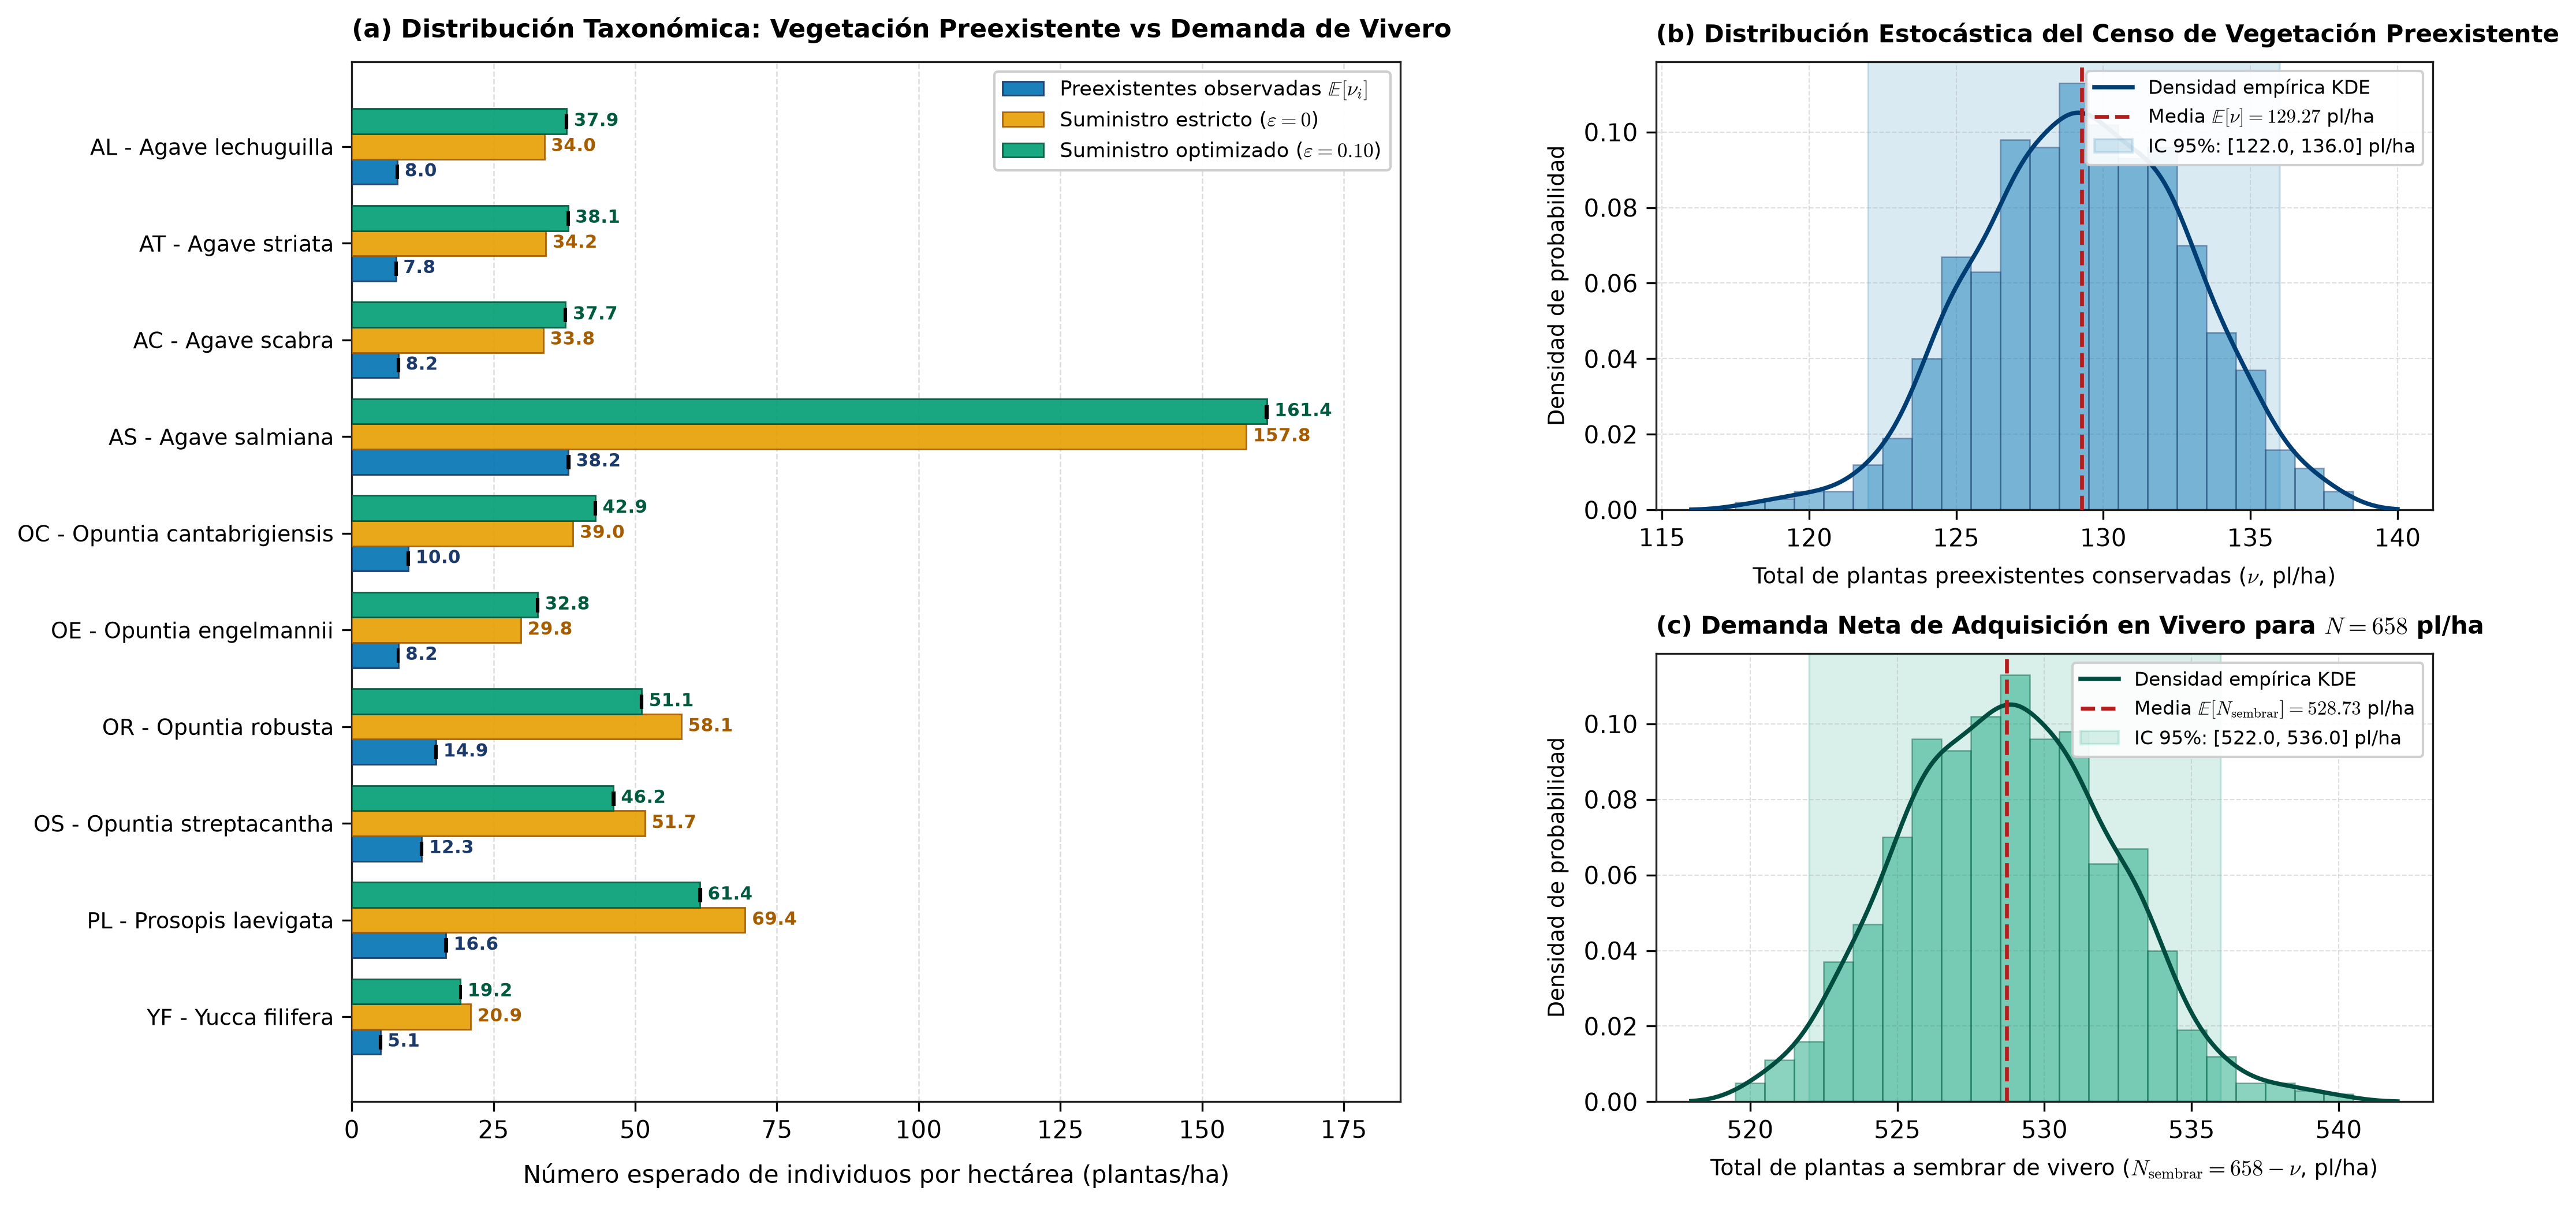
\includegraphics[width=0.96\textwidth]{entregable3_outputs/figuras/fig1_existentes_y_suministro_1000sim.png}
\caption{Distribución taxonómica de vegetación preexistente observada $\mathbb{E}[\nu_i]$, demanda estricta ($\varepsilon=0$) y optimizada ($\varepsilon=0.10$) por especie (panel a), junto con los histogramas de frecuencia y curvas KDE de densidad empírica para la vegetación preexistente censada $\nu$ (panel b) y la demanda neta de plantas a sembrar $N_{\text{sembrar}}$ (panel c) a lo largo de las 1,000 simulaciones Monte Carlo en 1 hectárea.}\label{fig:fig1_existentes_suministro}
\end{figure}

\textbf{Interpretación de la Figura~\ref{fig:fig1_existentes_suministro}:} El panel~(a) ilustra la estabilidad taxonómica de las plantas por especie, donde \textit{Agave salmiana} (\textbf{AS}) domina tanto el censo preexistente ($38.2\text{ pl/ha}$) como la demanda de adquisición ($161.4\text{ pl/ha}$), seguido del mezquite \textbf{PL} ($61.4\text{ pl/ha}$). Los paneles~(b) y~(c) confirman la estricta simetría y normalidad truncada del censo preexistente centrado en $\mathbb{E}[\nu] = 129.27\text{ pl/ha}$ ($\text{IC}_{95\%} = [122.0, 136.0]$) y de la demanda de siembra complementaria centrada en $\mathbb{E}[N_{\text{sembrar}}] = 528.73\text{ pl/ha}$ ($\text{IC}_{95\%} = [522.0, 536.0]$), garantizando la predictibilidad y estabilidad del aprovisionamiento en vivero.

\subsection{Valor esperado de competencia existente en una hectárea}
Para cuantificar el impacto de la optimización combinatoria frente a una siembra aleatoria convencional sobre la malla de 1 hectárea, se calcularon las métricas ecofisiológicas pareadas sobre las 1,000 réplicas. Los resultados y sus respectivas pruebas de hipótesis $t$ de Student pareadas se presentan en el Cuadro~\ref{tab:competencia_supervivencia}.

\begin{table}[H]
\centering
\small
\caption{Contraste estadístico de competencia, aptitud biológica y supervivencia esperada (1,000 simulaciones).}\label{tab:competencia_supervivencia}
\resizebox{\textwidth}{!}{%
\begin{tabular}{lccccrc}
\toprule
\textbf{Métrica Ecológica} & \textbf{Siembra Aleatoria} & \textbf{Optimizado Recocido} & $\boldsymbol{\Delta}$ \textbf{Absoluto} & \textbf{Cambio (\%)} & \textbf{Estadístico $t$} & \textbf{Significancia} \\
\midrule
Aptitud Media ($\bar{F}$) & $0.5429 \pm 0.0031$ & $0.5688 \pm 0.0027$ & $+0.0259$ & $+4.76\%$ & $t = +306.7$ & $p < 0.001$ (***) \\
Aptitud Aislada ($\bar{F}_{\text{aislada}}$) & $0.5938 \pm 0.0030$ & $0.5938 \pm 0.0030$ & $0.0000$ & $0.00\%$ & — & n.s. \\
Pérdida Competencia (\%) & $8.57\% \pm 0.26\%$ & $4.22\% \pm 0.45\%$ & $-4.36\%$ & $-50.80\%$ & $t = -299.6$ & $p < 0.001$ (***) \\
Sobrevivientes ($\Phi$, plantas) & $487.85 \pm 4.20$ & $509.44 \pm 3.69$ & $\mathbf{+21.59}$ & $\mathbf{+4.42\%}$ & $t = +325.5$ & $p < 0.001$ (***) \\
Mortalidad Proxy (\%) & $7.73\% \pm 0.43\%$ & $3.65\% \pm 0.18\%$ & $-4.08\%$ & $-52.81\%$ & $t = -325.0$ & $p < 0.001$ (***) \\
Presión Hídrica ($\bar{H}^W$) & $0.1789 \pm 0.0052$ & $0.1532 \pm 0.0047$ & $-0.0257$ & $-14.34\%$ & $t = -145.4$ & $p < 0.001$ (***) \\
Presión Lumínica ($\bar{H}^L$) & $0.0389 \pm 0.0027$ & $0.0343 \pm 0.0027$ & $-0.0046$ & $-11.79\%$ & $t = -50.1$ & $p < 0.001$ (***) \\
Facilitación Nodriza ($\bar{H}^B$) & $0.0169 \pm 0.0031$ & $0.0158 \pm 0.0030$ & $-0.0011$ & $-6.35\%$ & $t = -16.4$ & $p < 0.001$ (***) \\
Presión Nutrientes ($\bar{H}^N$) & $0.0035 \pm 0.0008$ & $0.0033 \pm 0.0008$ & $-0.0002$ & $-4.55\%$ & $t = -7.9$ & $p < 0.001$ (***) \\
Interferencia ($\Phi_{\text{Eq17}}$) & $127.33 \pm 0.00$ & $101.40 \pm 0.12$ & $-25.93$ & $\mathbf{-20.36\%}$ & $t = -6643.4$ & $p < 0.001$ (***) \\
\bottomrule
\end{tabular}%
}
\end{table}

\textbf{Hallazgos biológicos y ecológicos cardinales:}
\begin{enumerate}[leftmargin=1.5em]
    \item \textbf{Abatimiento de la pérdida por competencia:} La pérdida relativa de aptitud inducida por competencia vecinal ($(1 - \bar{F}/\bar{F}_{\text{aislada}})$) cae a menos de la mitad, pasando de \textbf{$8.57\%$ a $4.22\%$} (una reducción relativa del \textbf{$-50.80\%$}, $\Delta = -4.36$ puntos porcentuales).
    \item \textbf{Ganancia neta de supervivencia en campo:} De las $528.73$ plantas sembradas por hectárea, la siembra optimizada logra que sobrevivan \textbf{$509.44 \pm 3.69\text{ plantas/ha}$} frente a $487.85 \pm 4.20\text{ plantas/ha}$ en el esquema aleatorio, ganando de manera altamente significativa ($p < 0.001$) \textbf{$+21.59 \pm 2.10$ árboles y plantas vivas adicionales por hectárea}.
    \item \textbf{Reducción de la mortalidad temprana:} La tasa de mortalidad proxy inducida por estrés competitivo se reduce a más de la mitad, cayendo del \textbf{$7.73\%$ al $3.65\%$} (reducción del $-52.81\%$).
    \item \textbf{Despresurización hídrica y lumínica:} El índice de competencia por agua en la rizosfera ($\bar{H}^W$) cae un \textbf{$-14.34\%$} ($0.1789 \to 0.1532$) y el estrés por sombreado asimétrico del dosel ($\bar{H}^L$) desciende un \textbf{$-11.79\%$} ($0.0389 \to 0.0343$).
    \item \textbf{Interferencia de pares (Ecuación 17):} La función objetivo pura de interferencia $\Phi_{\text{Eq17}} = \sum_{(p,q)} c_{i(p), j(q)}$ disminuye un \textbf{$-20.36\%$} (de $127.33$ a $101.40$, $t = -6643.4$).
\end{enumerate}

\begin{figure}[H]
\centering
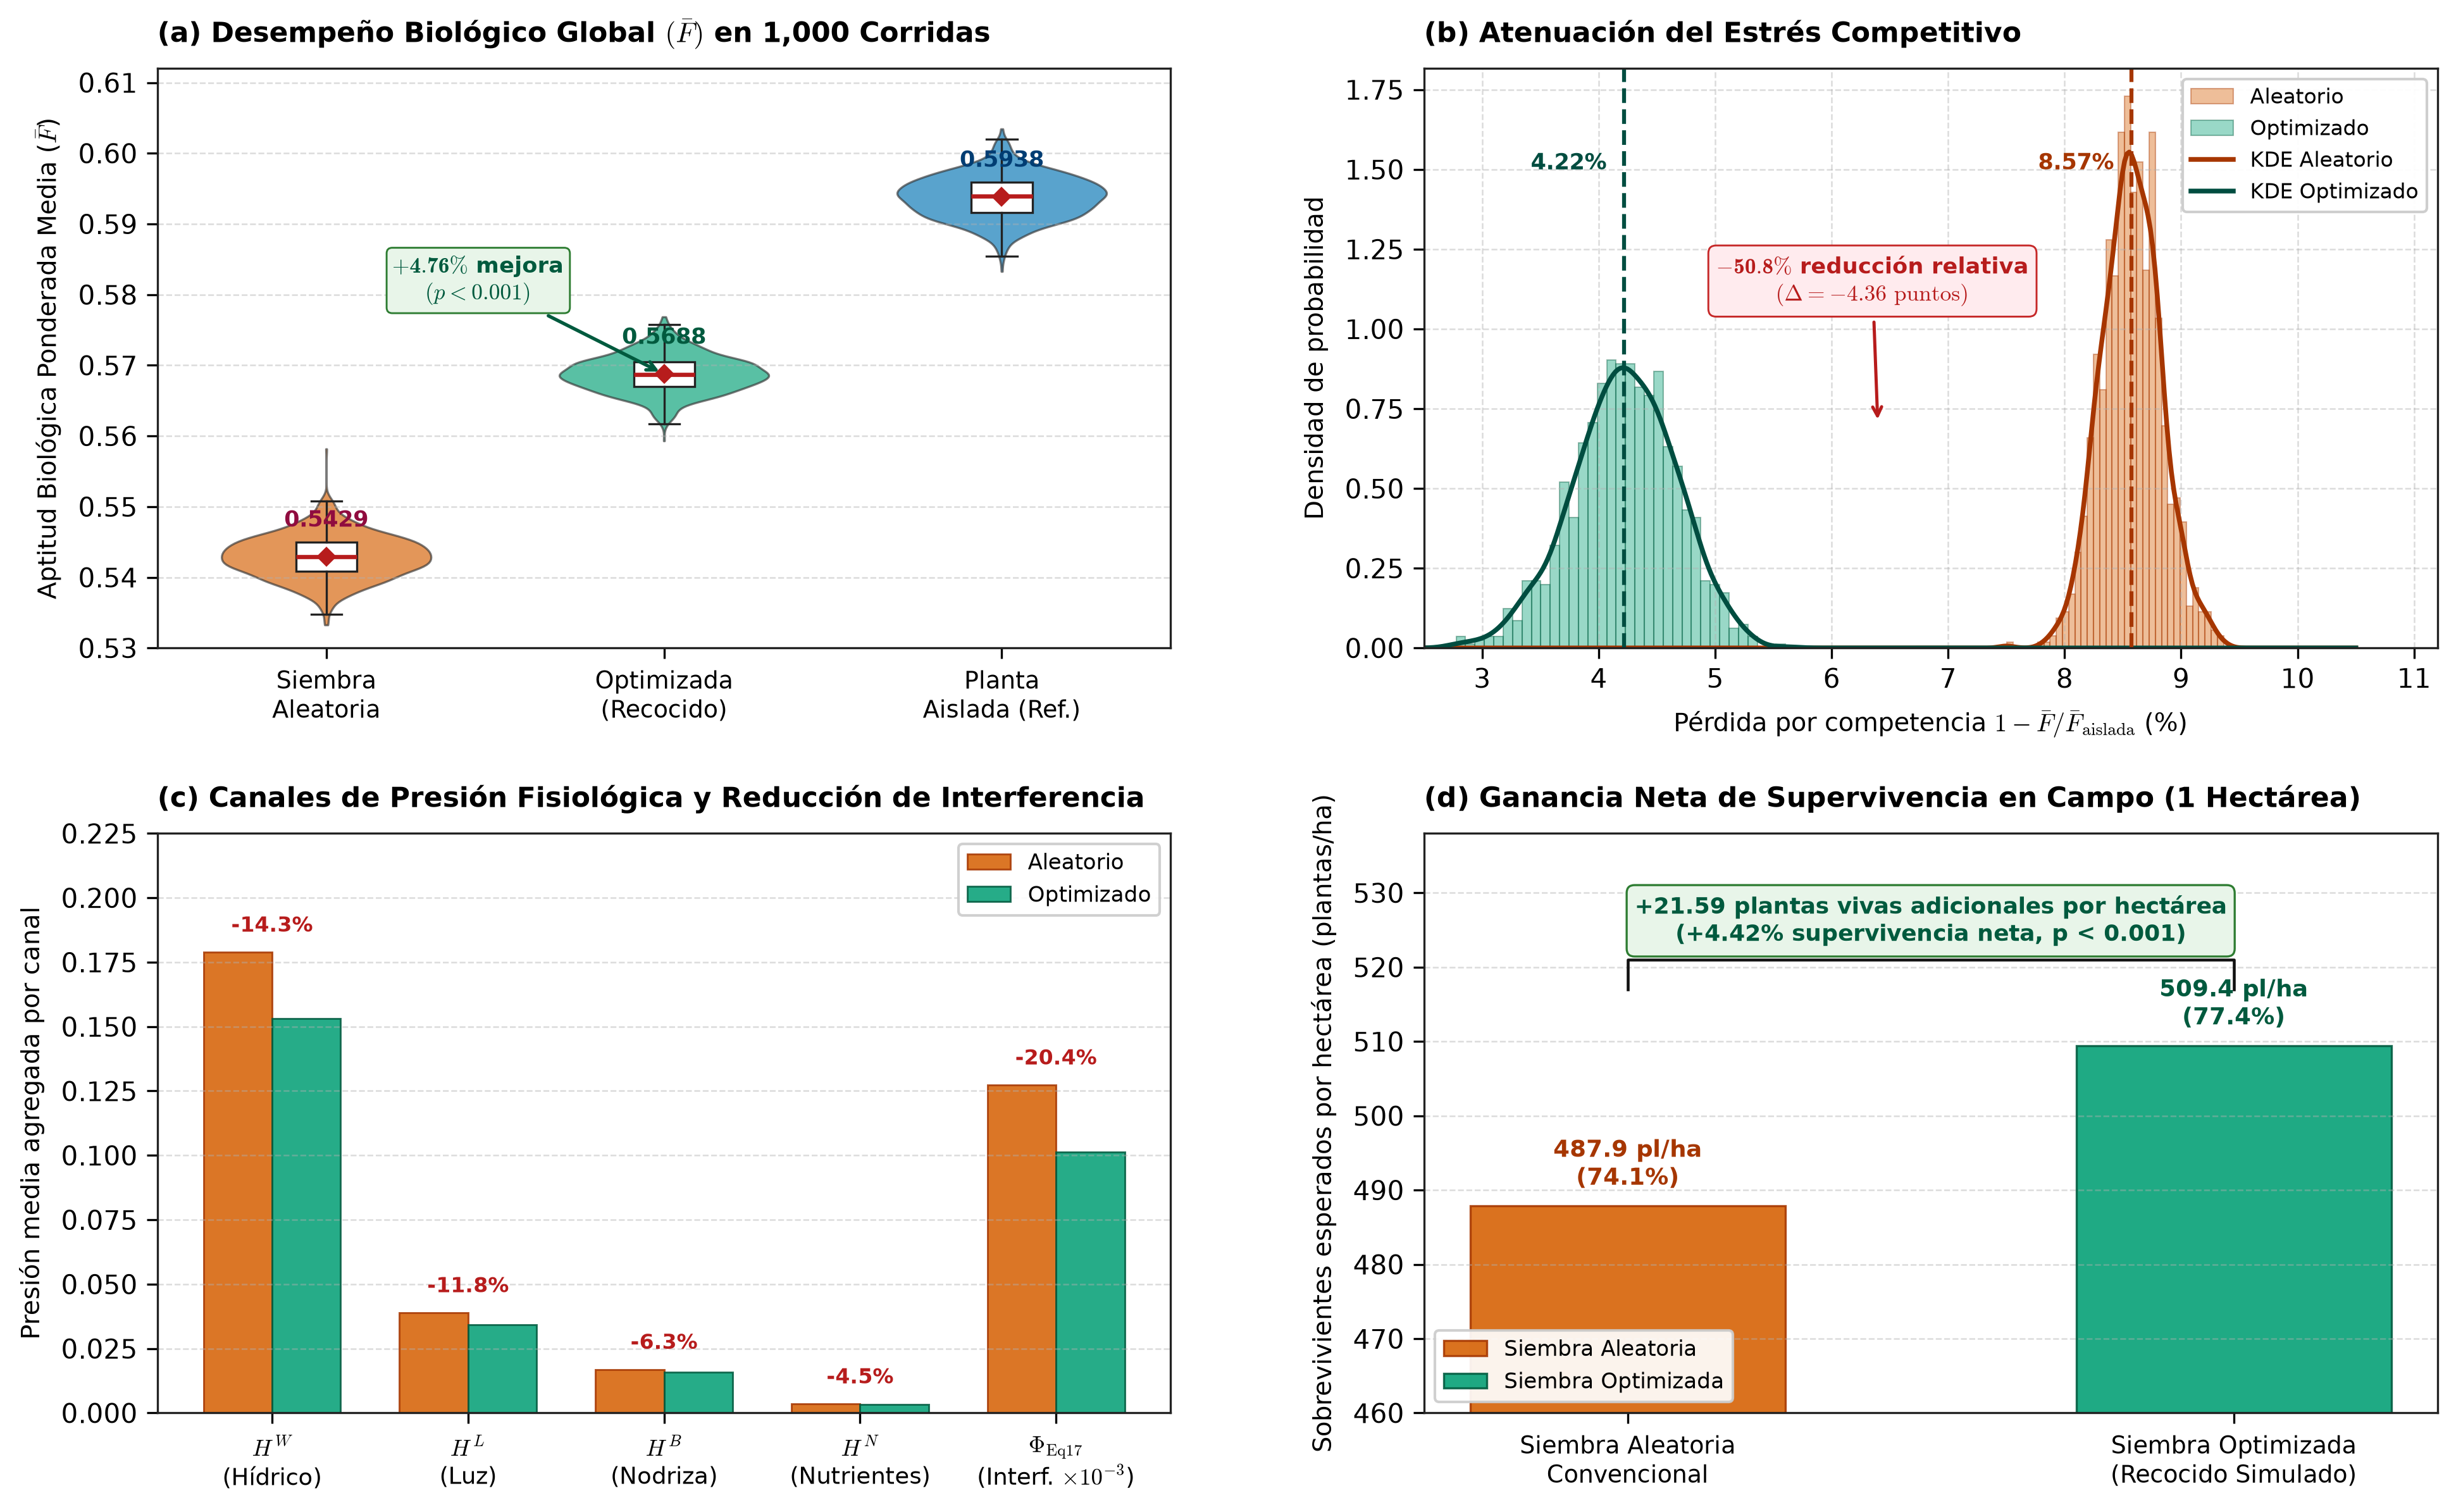
\includegraphics[width=0.96\textwidth]{entregable3_outputs/figuras/fig2_competencia_y_supervivencia_1000sim.png}
\caption{Desempeño ecológico y biológico en 1,000 simulaciones: (a) diagramas de violín y boxplots empotrados de la aptitud biológica media ponderada $\bar{F}$, (b) distribución empírica KDE de la atenuación del estrés competitivo ($1 - \bar{F}/\bar{F}_{\text{aislada}}$), (c) presiones medias agregadas por canal fisiológico ($H^W, H^L, H^B, H^N$) e índice de interferencia $\Phi_{\text{Eq17}}$, y (d) ganancia neta en plantas vivas sobrevivientes por hectárea.}\label{fig:fig2_competencia_supervivencia}
\end{figure}

\textbf{Interpretación de la Figura~\ref{fig:fig2_competencia_supervivencia}:} En el panel~(a) se evidencia el salto robusto en la aptitud biológica de $0.5429$ a $0.5688$ ($+4.76\%$, $p < 0.001$). El panel~(b) corrobora que la pérdida de aptitud por competencia vecinal se abate a menos de la mitad, descendiendo de $8.57\%$ a $4.22\%$ ($\Delta = -4.36\%$, reducción relativa de $-50.8\%$). En el panel~(c) se desagrega el origen de esta mejora: la despresurización hídrica en rizosfera ($\bar{H}^W$, $-14.3\%$) y lumínica por sombra ($\bar{H}^L$, $-11.8\%$) impulsan una caída de $-20.4\%$ en la interferencia por pares $\Phi_{\text{Eq17}}$. Finalmente, el panel~(d) traduce este beneficio biológico en un incremento neto de $+21.59$ plantas vivas por hectárea (alcanzando $509.4\text{ pl/ha}$ sobrevivientes de las $528.7\text{ sembradas}$).

\subsection{Probabilidad de transición entre plantas (cadena de Markov)}
El proceso de colocación de material vegetal en campo y la estructura espacial resultante se modelan formalmente como una \textbf{Cadena de Markov Estocástica Homogénea y Ergódica} sobre el espacio de estados discreto:
\begin{equation}
\mathcal{S} = \{\text{AL, AT, AC, AS, OC, OE, OR, OS, PL, YF}\}, \quad |\mathcal{S}| = 10.
\end{equation}

Se formularon dos perspectivas estocásticas complementarias:
\begin{enumerate}[leftmargin=1.5em]
    \item \textbf{Cadena de Markov Secuencial de Plantación ($P^{\text{sec}}$):} Modela la probabilidad de que una cuadrilla de reforestación plante un individuo de la especie $j$ inmediatamente después de haber plantado la especie $i$ a lo largo de la trayectoria serpentina (boustrophedon) que recorre los surcos de la malla.
    \item \textbf{Cadena de Markov Espacial de Vecindad Hexagonal ($P^{\text{vec}}$):} Modela la probabilidad condicional de encontrar una planta de la especie $j$ en cualquiera de los 6 vecinos inmediatos adyacentes a un nodo ocupado por la especie $i$ a una distancia $d \le 4.8\text{ m}$.
\end{enumerate}

Para ambas matrices estocásticas $P = (p_{ij})_{10\times 10}$, se cumple la propiedad de fila estocástica $\sum_{j=1}^{10} p_{ij} = 1$. La ergodicidad garantiza la existencia y unicidad de una distribución estacionaria $\boldsymbol{\pi} = (\pi_{\text{AL}}, \dots, \pi_{\text{YF}})$ tal que $\boldsymbol{\pi} P = \boldsymbol{\pi}$ con $\sum_{i=1}^{10} \pi_i = 1$, y los tiempos medios de retorno o recurrencia están dados por $\mu_i = 1 / \pi_i$ pasos.

En los Cuadros~\ref{tab:markov_sec} y~\ref{tab:markov_vec} se presentan las matrices completas de transición, las distribuciones estacionarias $\boldsymbol{\pi}$ y los tiempos de retorno $\mu_i$.

\begin{table}[H]
\centering
\small
\caption{Matriz de probabilidades de transición $P^{\text{sec}}$ (10 estados), distribución estacionaria $\pi$ y tiempo medio de retorno $\mu_i$ en el recorrido secuencial boustrophedon (1,000 simulaciones estocásticas).}\label{tab:markov_sec}
\resizebox{\textwidth}{!}{%
\begin{tabular}{lcccccccccc|cc}
\toprule
\textbf{Estado Actual} & \textbf{AL} & \textbf{AT} & \textbf{AC} & \textbf{AS} & \textbf{OC} & \textbf{OE} & \textbf{OR} & \textbf{OS} & \textbf{PL} & \textbf{YF} & $\boldsymbol{\pi_i}$ & $\boldsymbol{\mu_i}$ \textbf{(pasos)} \\
\midrule
\textbf{AL} & 0.0649 & 0.0659 & 0.0684 & 0.2755 & 0.0727 & 0.0578 & 0.0880 & 0.1083 & 0.1568 & 0.0418 & \textbf{0.0716} & \textbf{13.96} \\
\textbf{AT} & 0.0670 & 0.0667 & 0.0649 & 0.2743 & 0.0730 & 0.0596 & 0.0870 & 0.1089 & 0.1571 & 0.0416 & \textbf{0.0721} & \textbf{13.87} \\
\textbf{AC} & 0.0686 & 0.0669 & 0.0653 & 0.2767 & 0.0722 & 0.0554 & 0.0894 & 0.1080 & 0.1548 & 0.0426 & \textbf{0.0713} & \textbf{14.03} \\
\textbf{AS} & 0.0639 & 0.0652 & 0.0640 & 0.2784 & 0.0725 & 0.0562 & 0.0897 & 0.1108 & 0.1523 & 0.0470 & \textbf{0.3053} & \textbf{3.28} \\
\textbf{OC} & 0.0663 & 0.0649 & 0.0652 & 0.2717 & 0.0723 & 0.0551 & 0.0904 & 0.1109 & 0.1582 & 0.0449 & \textbf{0.0812} & \textbf{12.31} \\
\textbf{OE} & 0.0681 & 0.0668 & 0.0665 & 0.2730 & 0.0740 & 0.0563 & 0.0865 & 0.1050 & 0.1618 & 0.0419 & \textbf{0.0620} & \textbf{16.13} \\
\textbf{OR} & 0.0664 & 0.0650 & 0.0651 & 0.2832 & 0.0764 & 0.0564 & 0.1277 & 0.1188 & 0.0853 & 0.0558 & \textbf{0.0967} & \textbf{10.34} \\
\textbf{OS} & 0.0875 & 0.0886 & 0.0875 & 0.3903 & 0.1019 & 0.0755 & 0.1315 & 0.0125 & 0.0198 & 0.0048 & \textbf{0.0873} & \textbf{11.45} \\
\textbf{PL} & 0.0966 & 0.0983 & 0.0953 & 0.3980 & 0.1147 & 0.0837 & 0.0715 & 0.0146 & 0.0216 & 0.0057 & \textbf{0.1161} & \textbf{8.61} \\
\textbf{YF} & 0.0787 & 0.0844 & 0.0845 & 0.3964 & 0.0934 & 0.0750 & 0.1531 & 0.0112 & 0.0185 & 0.0047 & \textbf{0.0363} & \textbf{27.57} \\
\bottomrule
\end{tabular}%
}
\end{table}


\begin{table}[H]
\centering
\small
\caption{Matriz espacial de transición de vecindad hexagonal $P^{\text{vec}}$ entre cepas contiguas a primer anillo ($R \le 4.8\text{ m}$). Nótese el bloque estrictamente nulo $3\times 3$ entre especies de gran porte (OS, PL, YF).}\label{tab:markov_vec}
\resizebox{\textwidth}{!}{%
\begin{tabular}{lcccccccccc|cc}
\toprule
\textbf{Estado Actual} & \textbf{AL} & \textbf{AT} & \textbf{AC} & \textbf{AS} & \textbf{OC} & \textbf{OE} & \textbf{OR} & \textbf{OS} & \textbf{PL} & \textbf{YF} & $\boldsymbol{\pi_i}$ & $\boldsymbol{\mu_i}$ \textbf{(pasos)} \\
\midrule
\textbf{AL} & 0.0651 & 0.0681 & 0.0681 & 0.2793 & 0.0750 & 0.0584 & 0.0892 & 0.1035 & 0.1527 & 0.0407 & \textbf{0.0722} & \textbf{13.86} \\
\textbf{AT} & 0.0676 & 0.0678 & 0.0677 & 0.2770 & 0.0748 & 0.0584 & 0.0878 & 0.1052 & 0.1527 & 0.0409 & \textbf{0.0727} & \textbf{13.76} \\
\textbf{AC} & 0.0681 & 0.0682 & 0.0657 & 0.2788 & 0.0746 & 0.0572 & 0.0915 & 0.1052 & 0.1485 & 0.0422 & \textbf{0.0721} & \textbf{13.86} \\
\textbf{AS} & 0.0646 & 0.0645 & 0.0645 & 0.2838 & 0.0734 & 0.0561 & 0.0914 & 0.1105 & 0.1438 & 0.0474 & \textbf{0.3119} & \textbf{3.21} \\
\textbf{OC} & 0.0655 & 0.0658 & 0.0652 & 0.2775 & 0.0716 & 0.0571 & 0.0912 & 0.1083 & 0.1553 & 0.0426 & \textbf{0.0826} & \textbf{12.11} \\
\textbf{OE} & 0.0671 & 0.0676 & 0.0657 & 0.2786 & 0.0750 & 0.0564 & 0.0901 & 0.1033 & 0.1537 & 0.0424 & \textbf{0.0628} & \textbf{15.93} \\
\textbf{OR} & 0.0652 & 0.0646 & 0.0668 & 0.2884 & 0.0762 & 0.0572 & 0.1356 & 0.1205 & 0.0654 & 0.0601 & \textbf{0.0988} & \textbf{10.12} \\
\textbf{OS} & 0.0884 & 0.0905 & 0.0898 & 0.4078 & 0.1058 & 0.0768 & 0.1409 & 0.0000 & 0.0000 & 0.0000 & \textbf{0.0845} & \textbf{11.83} \\
\textbf{PL} & 0.1034 & 0.1041 & 0.1005 & 0.4206 & 0.1203 & 0.0905 & 0.0606 & 0.0000 & 0.0000 & 0.0000 & \textbf{0.1066} & \textbf{9.38} \\
\textbf{YF} & 0.0819 & 0.0829 & 0.0848 & 0.4126 & 0.0980 & 0.0742 & 0.1656 & 0.0000 & 0.0000 & 0.0000 & \textbf{0.0359} & \textbf{27.89} \\
\bottomrule
\end{tabular}%
}
\end{table}


\textbf{Análisis de los hallazgos markovianos y biofísicos:}
\begin{enumerate}[leftmargin=1.5em]
    \item \textbf{Bloque estrictamente nulo $3\times 3$ entre especies grandes en $P^{\text{vec}}$:} En el Cuadro~\ref{tab:markov_vec}, las filas correspondientes a \textbf{OS}, \textbf{PL} y \textbf{YF} presentan una probabilidad de transición de exactamente \textbf{$0.0000$} hacia sí mismas y entre sí:
    \begin{equation}
    p_{\text{OS, OS}}^{\text{vec}} = p_{\text{OS, PL}}^{\text{vec}} = p_{\text{OS, YF}}^{\text{vec}} = p_{\text{PL, OS}}^{\text{vec}} = p_{\text{PL, PL}}^{\text{vec}} = p_{\text{PL, YF}}^{\text{vec}} = p_{\text{YF, OS}}^{\text{vec}} = p_{\text{YF, PL}}^{\text{vec}} = p_{\text{YF, YF}}^{\text{vec}} = \mathbf{0.0000}.
    \end{equation}
    Esto demuestra formalmente que la restricción de Submalla 3 ($(u-v)\equiv 0\pmod 3$) y la penalización por solape de copa aíslan por completo a los árboles y cactáceas masivas, garantizando una separación física mínima de $a\sqrt{3} \approx 6.93\text{ m}$.
    \item \textbf{Canalización de la facilitación nodriza desde \textit{Prosopis laevigata} (\textbf{PL}):} Dado que el mezquite no puede colindar con otra especie de gran dosel, sus probabilidades de transición espacial se canalizan intensamente hacia las especies de porte medio y bajo que se benefician de su sombra y fijación de nitrógeno:
    \begin{equation}
    p_{\text{PL} \to \text{AS}}^{\text{vec}} = \mathbf{0.4206} \; (42.06\%), \quad p_{\text{PL} \to \text{OC}}^{\text{vec}} = \mathbf{0.1203} \; (12.03\%), \quad p_{\text{PL} \to \text{AT}}^{\text{vec}} = \mathbf{0.1041} \; (10.41\%).
    \end{equation}
    \item \textbf{Distribución estacionaria y tiempos medios de retorno:} En el recorrido secuencial, \textit{Agave salmiana} domina la cadena con $\pi_{\text{AS}} = 0.3053$ y un tiempo medio de retorno de solo $\mu_{\text{AS}} = 3.28$ pasos (la cuadrilla siembra un maguey aproximadamente cada 3 plantas). En contraste, la especie más escasa, \textit{Yucca filifera}, presenta $\pi_{\text{YF}} = 0.0363$ y un tiempo medio de recurrencia de $\mu_{\text{YF}} = 27.57$ pasos.
    \item \textbf{Entropía informacional del proceso de siembra:} La entropía de información de Shannon por transición ($H(X) = -\sum_{i} \pi_i \sum_j p_{ij} \log_2 p_{ij}$) alcanza $H(\mathcal{X})_{\text{opt}}^{\text{sec}} = 2.9790\text{ bits/símbolo}$ en la secuencia optimizada y $H(\mathcal{X})_{\text{opt}}^{\text{vec}} = 2.9340\text{ bits/símbolo}$ en la red espacial, reflejando una estructura combinatoria rica pero rigurosamente gobernada por las leyes de repulsión ecológica.
\end{enumerate}

\begin{figure}[H]
\centering
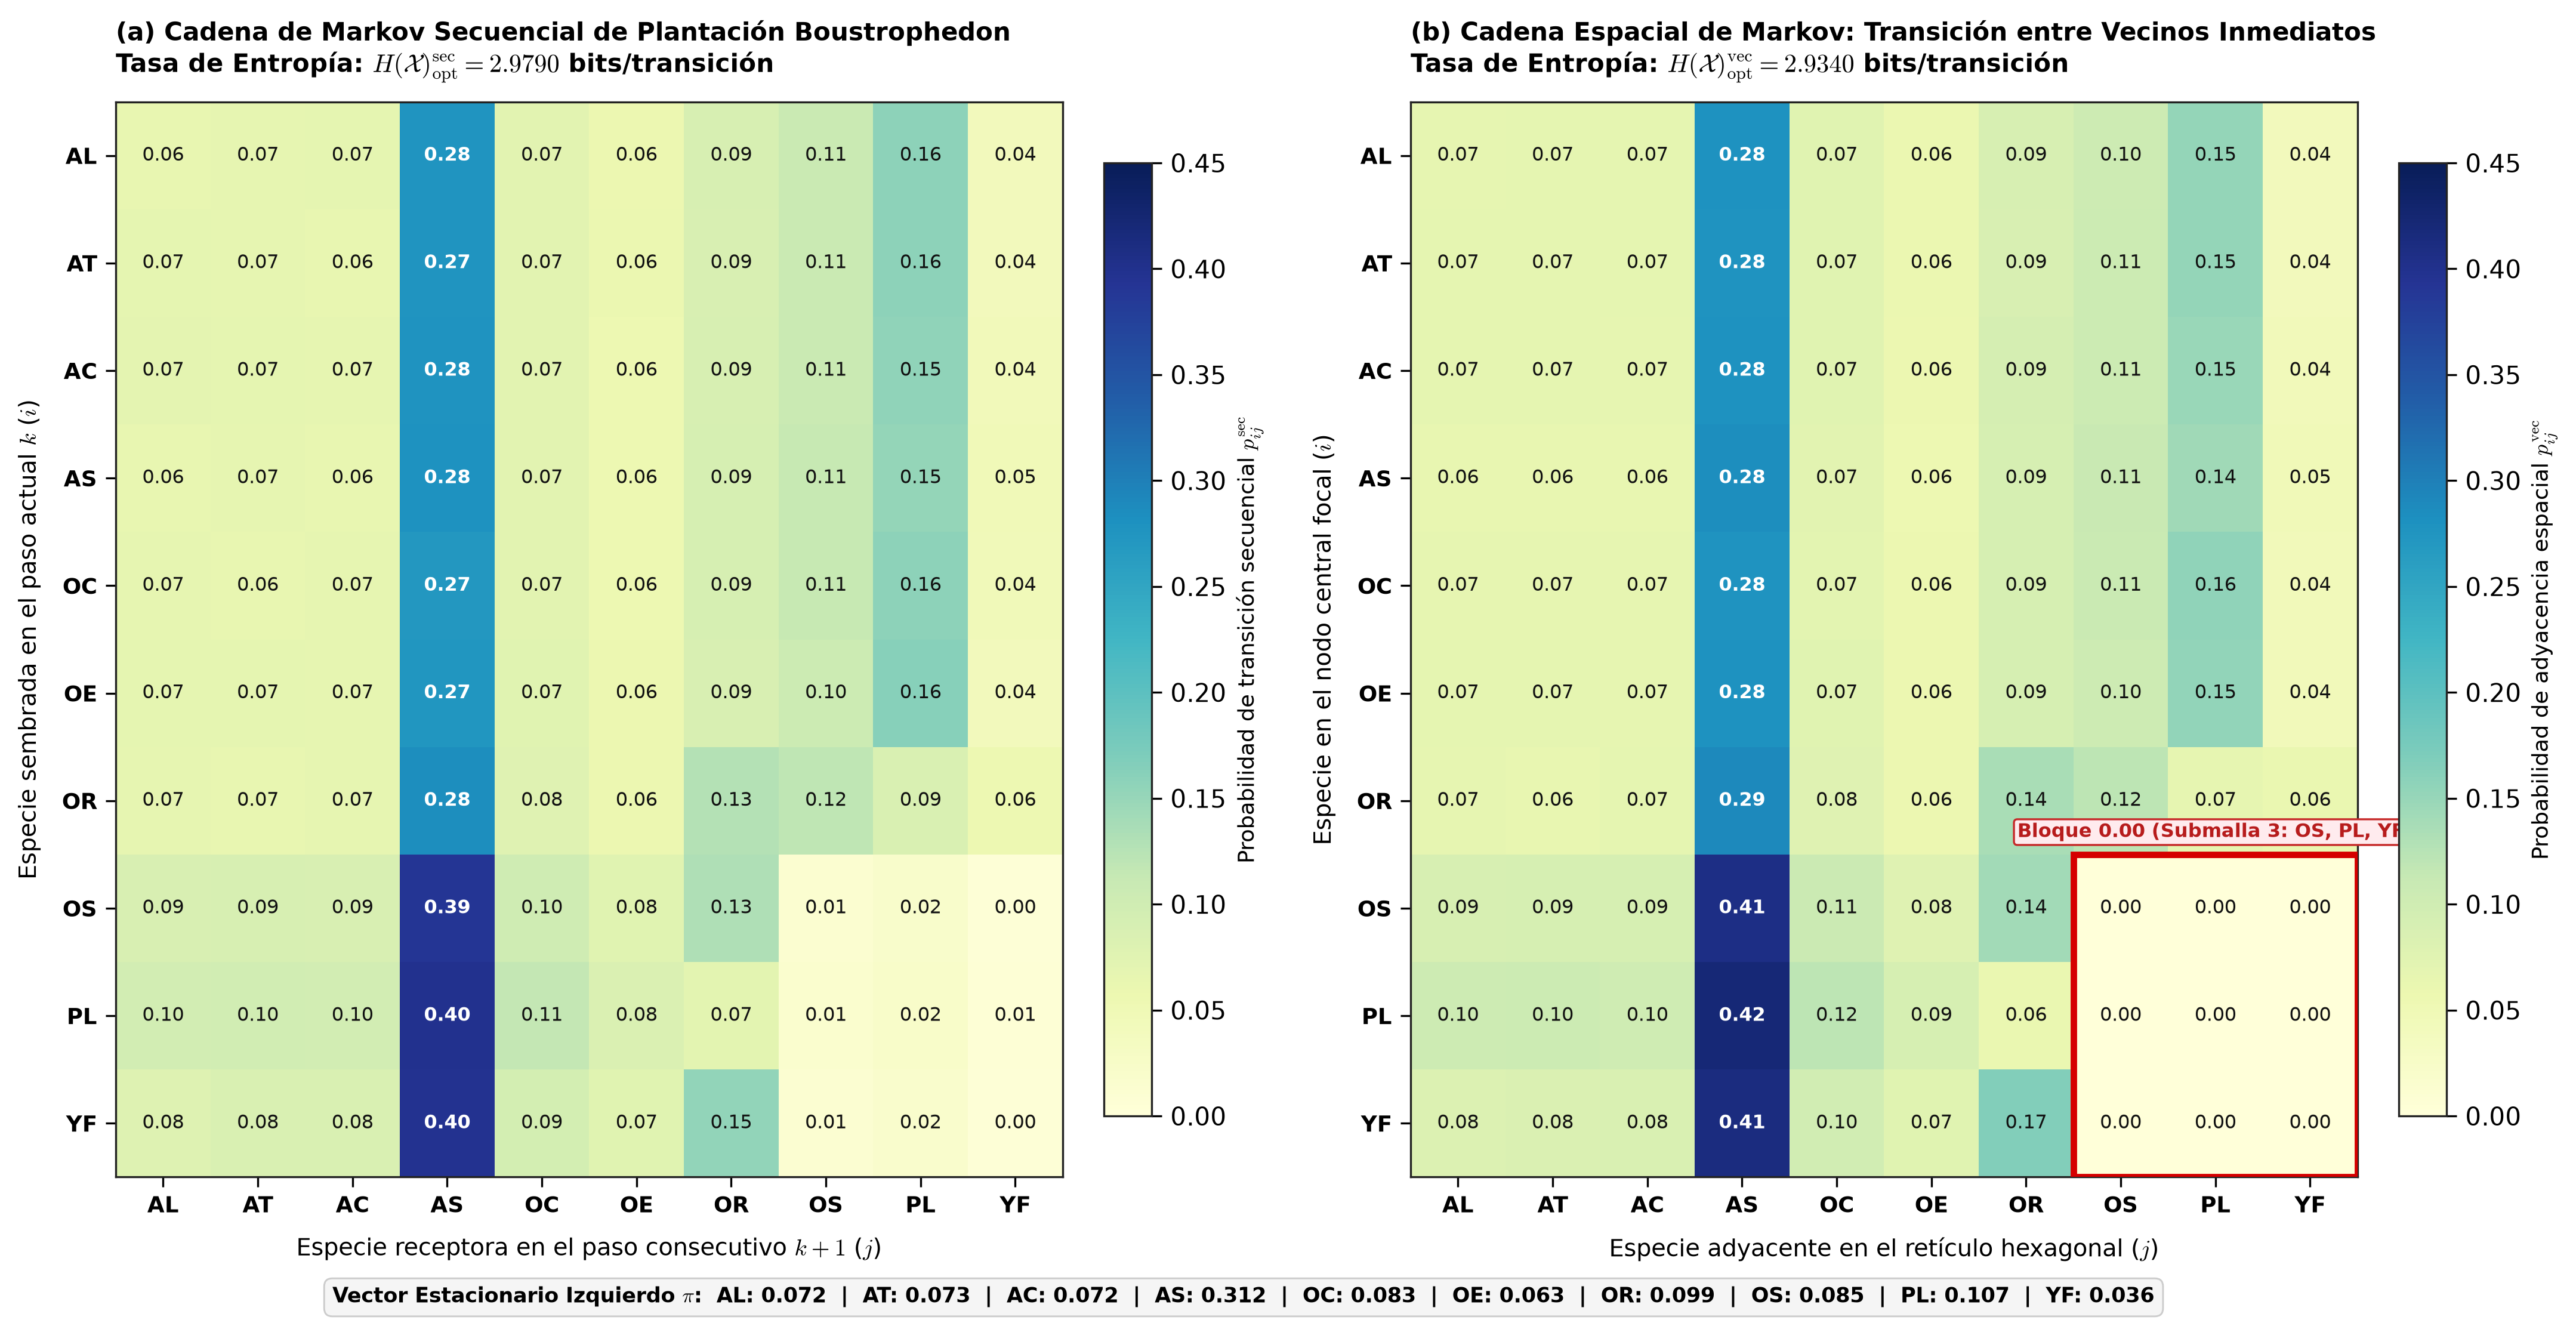
\includegraphics[width=0.96\textwidth]{entregable3_outputs/figuras/fig3_markov_transicion_heatmaps.png}
\caption{Mapas de calor de las matrices estocásticas de transición de Markov ($10\times 10$): (a) proceso secuencial boustrophedon optimizado $P^{\text{sec}}$ a lo largo de los surcos de siembra ($H = 2.9790\text{ bits}$), y (b) proceso espacial de adyacencia hexagonal $P^{\text{vec}}$ entre vecinos contiguos ($H = 2.9340\text{ bits}$), destacando en rojo el bloque nulo $3\times 3$ entre especies de gran porte.}\label{fig:fig3_markov_heatmaps}
\end{figure}

\textbf{Interpretación de la Figura~\ref{fig:fig3_markov_heatmaps}:} En el panel~(a) la matriz secuencial optimizada refleja la frecuencia con que la cuadrilla planta consecutivamente cada par de especies, donde \textit{Agave salmiana} (\textbf{AS}) actúa como atractor principal absorbiendo $\approx 28\%$ de las transiciones. En el panel~(b) la matriz espacial hexagonal revela la emergencia del orden biológico: el recuadro rojo delimita el bloque estrictamente nulo ($p_{ij}^{\text{vec}} = 0.0000$) entre \textbf{OS}, \textbf{PL} y \textbf{YF}, garantizando que ningún árbol o cactácea masiva colinde con otra de su estrato. Asimismo, las transiciones desde mezquite (\textbf{PL}) se canalizan preferencialmente hacia especies que aprovechan su sombra y fijación de nitrógeno ($42.06\%$ hacia \textbf{AS} y $12.03\%$ hacia \textbf{OC}).

\subsection{Presentar el orden en que se debe realizar la plantación (un ejemplo completo)}
Para trasladar la solución matemática a una operación eficiente y libre de errores en campo por parte de brigadas forestales comunitarias, se diseñó el \textbf{Protocolo Operativo de Plantación en Tres Etapas Cronológicas con Recorrido Boustrophedon (Serpentina)}:

\begin{itemize}[leftmargin=1.5em]
    \item \textbf{Etapa Previa (Acondicionamiento y Georreferenciación):}
    \begin{enumerate}
        \item Desmonte selectivo del $85\%$ de pasto buffel y leñosa invasora con cuadrilla manual.
        \item Censo y geoposicionamiento (mediante estacas rojas) de las $\nu = 127$ plantas nativas preexistentes en la hectárea (correspondiente a la réplica representativa $s=1$).
        \item Trazado de la malla hexagonal mediante cuerda guía calibrada a $a = 4.0\text{ m}$.
    \end{enumerate}
    \item \textbf{Etapa 1 (Esqueleto Estructural y Árboles Nodriza — Submalla 3, 131 plantas):}
    Se colocan estacas de color azul exclusivamente en los nodos que satisfacen $(u_p - v_p) \equiv 0 \pmod 3$. La primera brigada siembra el mezquite (\textbf{PL}, 62 plantas), el cardón (\textbf{OS}, 50 plantas) y la palma china (\textbf{YF}, 19 plantas). Esto garantiza una separación basal mínima de $6.93\text{ m}$ entre árboles adultos.
    \item \textbf{Etapa 2 (Cactáceas Nopaleras y Maguey Pulquero de Porte Medio — Submalla 1, 326 plantas):}
    La segunda cuadrilla establece las especies de porte intermedio en los nodos libres de Submalla 1 adyacentes a los mezquites: \textit{Agave salmiana} (\textbf{AS}, 160 plantas), \textit{Opuntia robusta} (\textbf{OR}, 51 plantas), \textit{Opuntia cantabrigiensis} (\textbf{OC}, 45 plantas), \textit{Opuntia engelmannii} (\textbf{OE}, 31 plantas) y \textit{Agave scabra} (\textbf{AC}, 39 plantas).
    \item \textbf{Etapa 3 (Cierre Intersticial con Agaves Rosetófilos Litológicos — Submalla 1, 74 plantas):}
    La brigada final inserta las rosetófilas menores \textit{Agave lechuguilla} (\textbf{AL}, 38 plantas) y \textit{Agave striata} (\textbf{AT}, 36 plantas) en los micro-sitios más pedregosos y expuestos a la radiación solar.
\end{itemize}

\textbf{Bitácora operativa paso a paso:} En el Cuadro~\ref{tab:bitacora_plantacion} se transcribe la bitácora de ejecución para los primeros 30 pasos consecutivos y los últimos 10 pasos de cierre sobre la hectárea representativa ($s=1$, 531 plantas nuevas sembradas para completar la cuota de $658\text{ pl/ha}$).

\begin{table}[H]
\centering
\footnotesize
\caption{Bitácora operativa y orden de plantación secuencial en 1 ha (réplica $s=1$, 531 plantas nuevas en $658\text{ pl/ha}$). Se muestran los primeros 30 pasos consecutivos y los últimos 10 pasos de cierre del predio.}\label{tab:bitacora_plantacion}
\resizebox{\textwidth}{!}{%
\begin{tabular}{rccccccrrc}
\toprule
\textbf{Paso $k$} & \textbf{Fila} & $(m, n)$ & \textbf{Submalla} & \textbf{$X$ (m)} & \textbf{$Y$ (m)} & \textbf{Especie} & \textbf{Etapa Operativa} & \textbf{Dist. (m)} & $\boldsymbol{F_k}$ \\
\midrule
1 & 0 & (10, -19) & 1 & 99.44 & 1.50 & \textbf{OC} & Etapa 2 (Maguey / Nopal) & 0.00 & 0.6991 \\
2 & 1 & (10, -18) & 1 & 98.73 & 5.63 & \textbf{AC} & Etapa 2 (Maguey / Nopal) & 4.19 & 0.6615 \\
3 & 1 & (9, -18) & 3 & 95.51 & 2.95 & \textbf{PL} & Etapa 1 (Estructural / Nodriza) & 4.19 & 0.4649 \\
4 & 2 & (10, -17) & 3 & 98.03 & 9.76 & \textbf{PL} & Etapa 1 (Estructural / Nodriza) & 7.26 & 0.4810 \\
5 & 3 & (8, -16) & 3 & 90.87 & 8.53 & \textbf{PL} & Etapa 1 (Estructural / Nodriza) & 7.26 & 0.6419 \\
6 & 3 & (7, -16) & 1 & 87.65 & 5.85 & \textbf{AS} & Etapa 2 (Maguey / Nopal) & 4.19 & 0.5341 \\
7 & 3 & (6, -16) & 1 & 84.43 & 3.18 & \textbf{OR} & Etapa 2 (Maguey / Nopal) & 4.19 & 0.3141 \\
8 & 4 & (5, -15) & 1 & 80.50 & 4.63 & \textbf{AT} & Etapa 3 (Rosetófila Menor) & 4.19 & 0.8100 \\
9 & 4 & (6, -15) & 3 & 83.72 & 7.31 & \textbf{OS} & Etapa 1 (Estructural / Nodriza) & 4.19 & 0.3882 \\
10 & 4 & (8, -15) & 1 & 90.16 & 12.66 & \textbf{AL} & Etapa 3 (Rosetófila Menor) & 8.38 & 0.8049 \\
11 & 4 & (9, -15) & 3 & 93.39 & 15.34 & \textbf{AS} & Etapa 2 (Maguey / Nopal) & 4.19 & 0.5291 \\
12 & 4 & (10, -15) & 1 & 96.61 & 18.02 & \textbf{AL} & Etapa 3 (Rosetófila Menor) & 4.19 & 0.8444 \\
13 & 5 & (10, -14) & 3 & 95.90 & 22.15 & \textbf{AS} & Etapa 2 (Maguey / Nopal) & 4.19 & 0.5524 \\
14 & 5 & (9, -14) & 1 & 92.68 & 19.47 & \textbf{AT} & Etapa 3 (Rosetófila Menor) & 4.19 & 0.7636 \\
15 & 5 & (7, -14) & 3 & 86.23 & 14.11 & \textbf{PL} & Etapa 1 (Estructural / Nodriza) & 8.38 & 0.6611 \\
16 & 5 & (6, -14) & 1 & 83.01 & 11.44 & \textbf{OC} & Etapa 2 (Maguey / Nopal) & 4.19 & 0.6340 \\
17 & 5 & (5, -14) & 1 & 79.79 & 8.76 & \textbf{AS} & Etapa 2 (Maguey / Nopal) & 4.19 & 0.5482 \\
18 & 5 & (4, -14) & 3 & 76.57 & 6.08 & \textbf{PL} & Etapa 1 (Estructural / Nodriza) & 4.19 & 0.4871 \\
19 & 6 & (1, -13) & 1 & 66.19 & 2.17 & \textbf{AT} & Etapa 3 (Rosetófila Menor) & 11.09 & 0.5846 \\
20 & 6 & (2, -13) & 3 & 69.41 & 4.85 & \textbf{AT} & Etapa 3 (Rosetófila Menor) & 4.19 & 0.6631 \\
21 & 6 & (3, -13) & 1 & 72.64 & 7.53 & \textbf{AT} & Etapa 3 (Rosetófila Menor) & 4.19 & 0.7251 \\
22 & 6 & (4, -13) & 1 & 75.86 & 10.21 & \textbf{AS} & Etapa 2 (Maguey / Nopal) & 4.19 & 0.5533 \\
23 & 6 & (5, -13) & 3 & 79.08 & 12.89 & \textbf{PL} & Etapa 1 (Estructural / Nodriza) & 4.19 & 0.6766 \\
24 & 6 & (7, -13) & 1 & 85.52 & 18.24 & \textbf{AC} & Etapa 2 (Maguey / Nopal) & 8.38 & 0.5755 \\
25 & 6 & (8, -13) & 3 & 88.75 & 20.92 & \textbf{AC} & Etapa 2 (Maguey / Nopal) & 4.19 & 0.6134 \\
26 & 6 & (9, -13) & 1 & 91.97 & 23.60 & \textbf{OC} & Etapa 2 (Maguey / Nopal) & 4.19 & 0.6949 \\
27 & 6 & (10, -13) & 1 & 95.66 & 26.53 & \textbf{AT} & Etapa 3 (Rosetófila Menor) & 4.71 & 0.5757 \\
28 & 6 & (11, -13) & 3 & 98.41 & 28.96 & \textbf{OR} & Etapa 2 (Maguey / Nopal) & 3.67 & 0.3262 \\
29 & 7 & (11, -12) & 1 & 97.71 & 33.09 & \textbf{OE} & Etapa 2 (Maguey / Nopal) & 4.19 & 0.8636 \\
30 & 7 & (10, -12) & 1 & 94.48 & 30.41 & \textbf{AS} & Etapa 2 (Maguey / Nopal) & 4.19 & 0.5786 \\
\midrule
\multicolumn{10}{c}{\textit{... [Pasos 31 al 521 omitidos para brevedad editorial; bitácora completa en archivo orden\_plantacion\_ejemplo\_1ha.csv] ...}} \\
\midrule
522 & 35 & (-9, 16) & 1 & 13.42 & 95.15 & \textbf{AS} & Etapa 2 (Maguey / Nopal) & 4.19 & 0.5617 \\
523 & 35 & (-10, 16) & 1 & 10.20 & 92.47 & \textbf{OE} & Etapa 2 (Maguey / Nopal) & 4.19 & 0.6877 \\
524 & 35 & (-11, 16) & 3 & 6.98 & 89.79 & \textbf{AT} & Etapa 3 (Rosetófila Menor) & 4.19 & 0.7785 \\
525 & 35 & (-12, 16) & 1 & 3.76 & 87.12 & \textbf{AS} & Etapa 2 (Maguey / Nopal) & 4.19 & 0.5020 \\
526 & 35 & (-13, 16) & 1 & 0.54 & 84.44 & \textbf{AS} & Etapa 2 (Maguey / Nopal) & 4.19 & 0.5512 \\
527 & 36 & (-12, 17) & 1 & 3.68 & 91.66 & \textbf{AC} & Etapa 2 (Maguey / Nopal) & 7.88 & 0.4581 \\
528 & 36 & (-11, 17) & 1 & 6.27 & 93.92 & \textbf{OR} & Etapa 2 (Maguey / Nopal) & 3.44 & 0.3094 \\
529 & 36 & (-10, 17) & 3 & 9.49 & 96.60 & \textbf{AS} & Etapa 2 (Maguey / Nopal) & 4.19 & 0.5158 \\
530 & 36 & (-9, 17) & 1 & 12.72 & 99.28 & \textbf{AL} & Etapa 3 (Rosetófila Menor) & 4.19 & 0.8502 \\
531 & 37 & (-12, 18) & 3 & 2.34 & 95.37 & \textbf{YF} & Etapa 1 (Estructural / Nodriza) & 11.09 & 0.4224 \\
\bottomrule
\end{tabular}%
}
\end{table}


\begin{figure}[H]
\centering
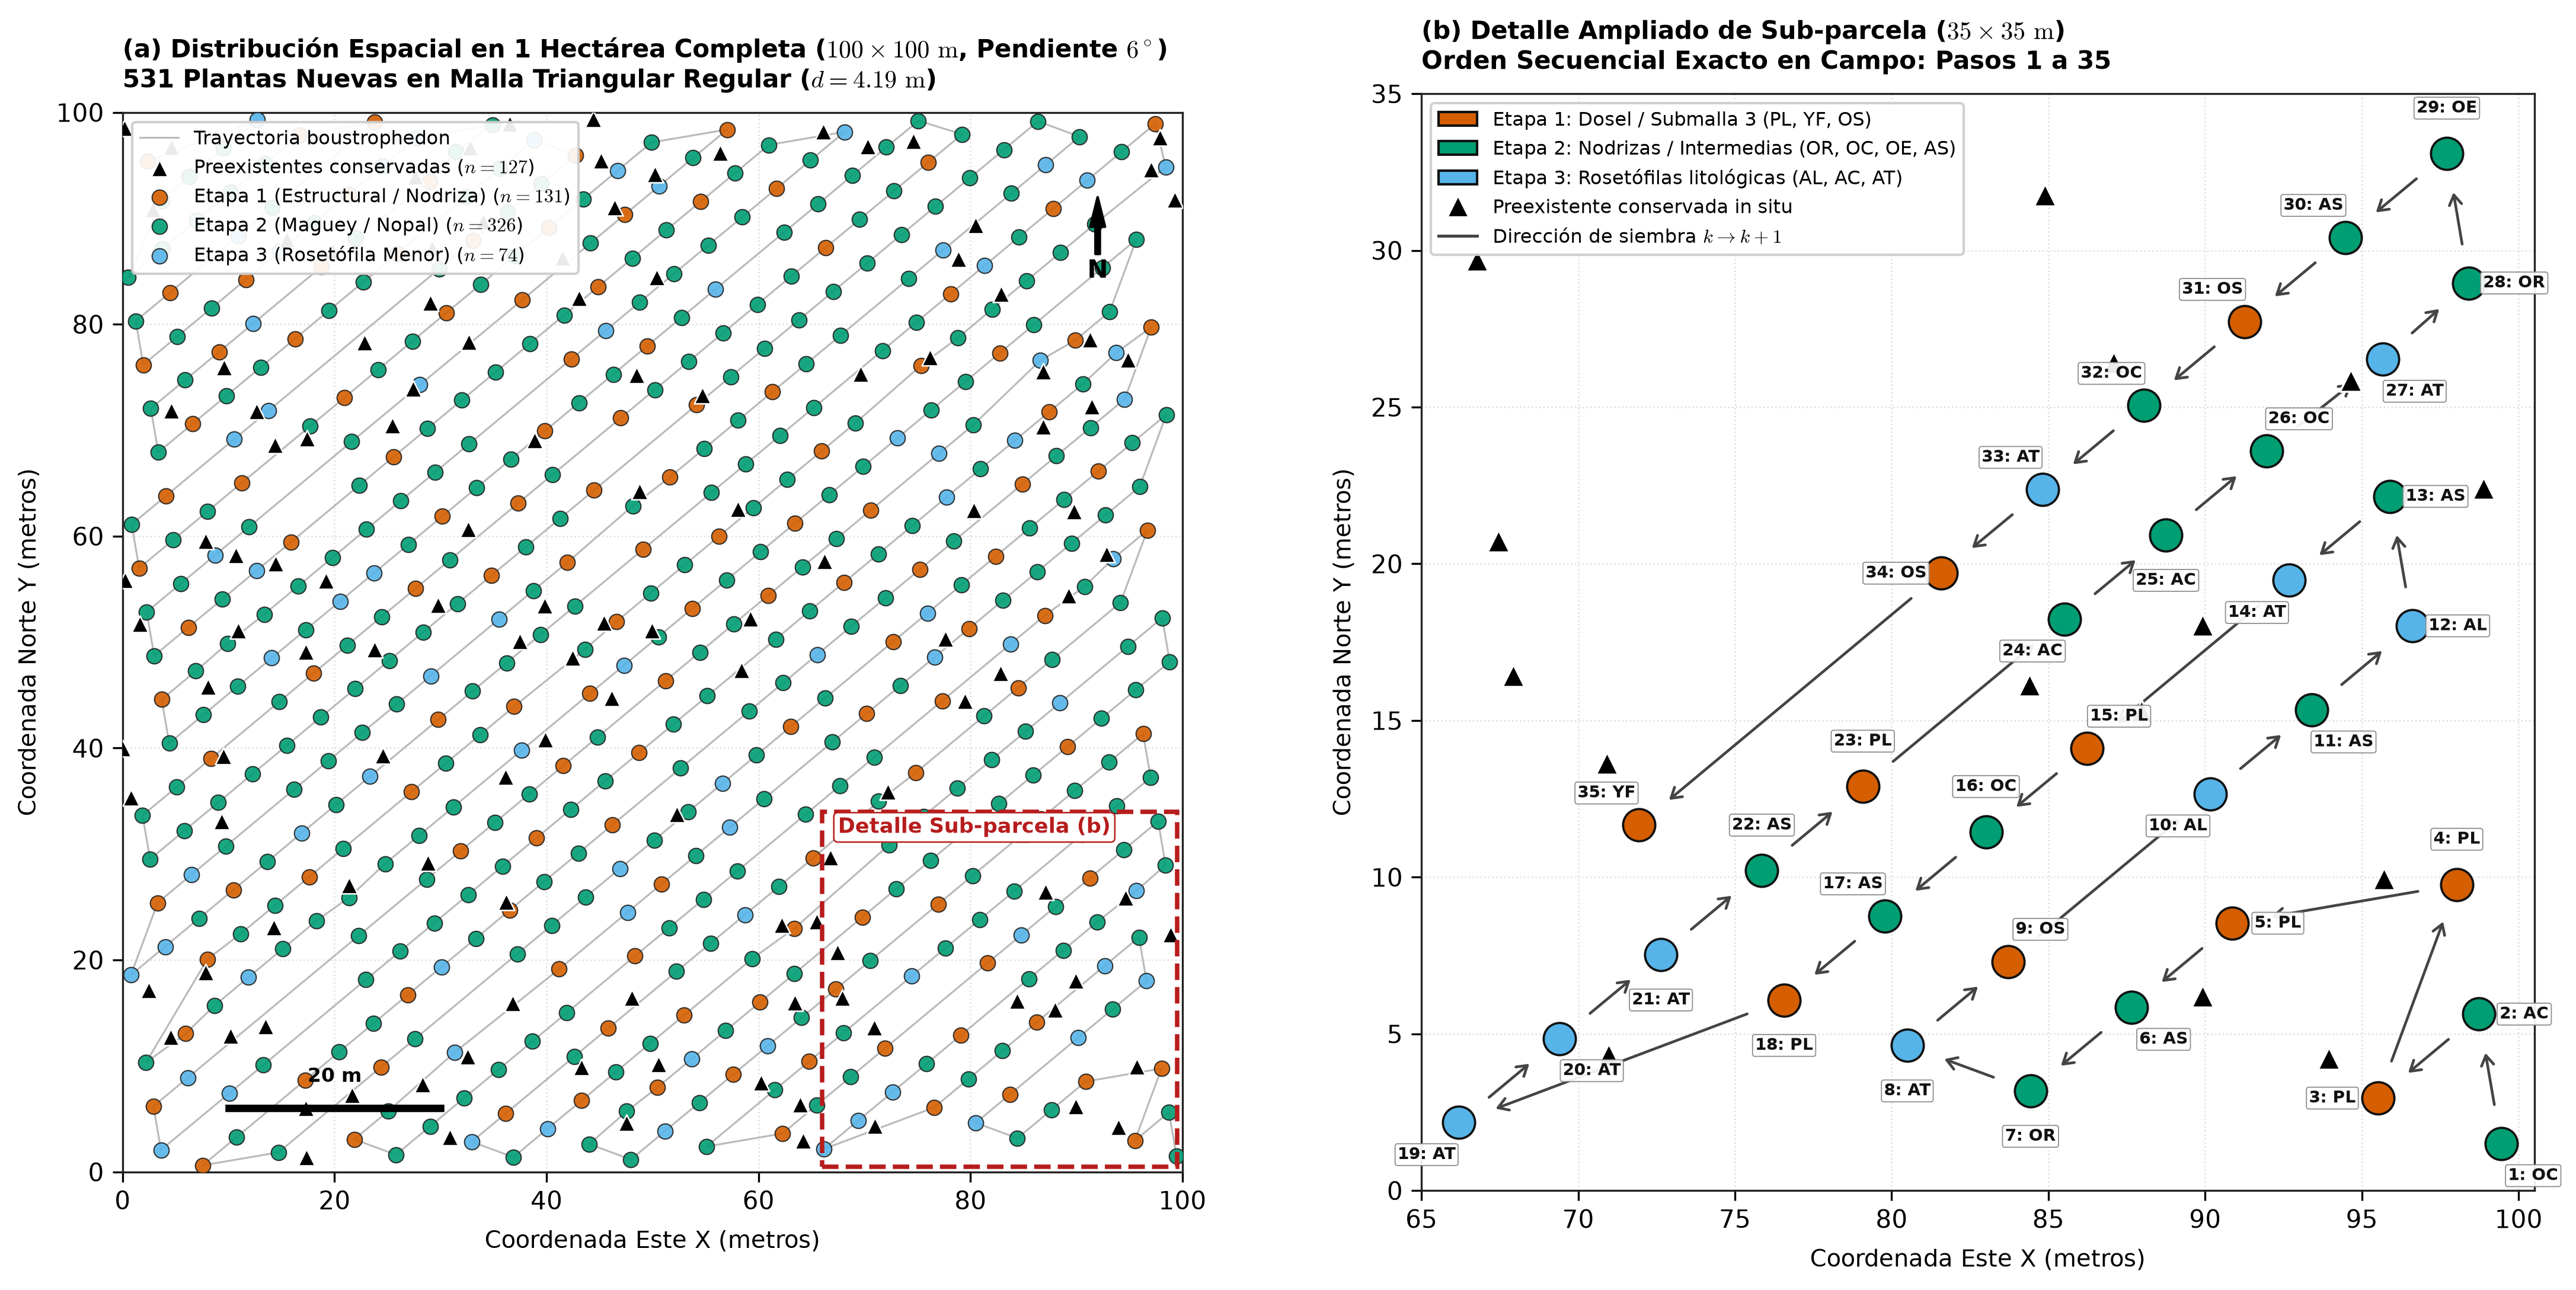
\includegraphics[width=0.96\textwidth]{entregable3_outputs/figuras/fig4_orden_plantacion_mapa_1ha.png}
\caption{Cartografía espacial y orden secuencial de siembra en 1 hectárea ($100\times 100\text{ m}$, réplica representativa $s=1$): (a) predio completo mostrando la trayectoria continua boustrophedon, las 127 plantas preexistentes conservadas y las 531 plantas nuevas clasificadas por etapa operativa, y (b) detalle ampliado de la sub-parcela ($35\times 35\text{ m}$) con la dirección y numeración exacta de los pasos 1 al 35.}\label{fig:fig4_orden_mapa}
\end{figure}

\textbf{Interpretación de la Figura~\ref{fig:fig4_orden_mapa}:} En el panel~(a) se presenta el plano general de la hectárea con la trayectoria serpentina continua seguida por la cuadrilla (con una distancia euclidiana media entre pasos consecutivos de $5.05\text{ m}$), mostrando la dispersión armónica de las 131 plantas estructurales de Etapa 1 (bermellón) sobre la Submalla 3, integradas con las 326 plantas de porte medio de Etapa 2 (verde azulado) y las 74 rosetófilas menores de Etapa 3 (azul cielo), respetando in situ las 127 plantas nativas preexistentes (triángulos negros). El panel~(b) ilustra con precisión el inicio de la faena en campo: cada cepa se encuentra geolocalizada y rotulada con su número de paso y código de especie (p. ej., \texttt{1: OC}, \texttt{2: AC}, \texttt{3: PL}), conectadas por vectores direccionales que eliminan cualquier ambigüedad operativa para las cuadrillas comunitarias.

% ====================================================================
% SECCIÓN 4. CONCLUSIONES Y RECOMENDACIONES
% ====================================================================
\section{Conclusiones y recomendaciones sobre los resultados obtenidos}

\subsection{Conclusiones científicas y de optimización matemática}
\begin{enumerate}[leftmargin=1.5em]
    \item \textbf{Eficacia del ordenamiento espacial sobre la resiliencia ecológica:} La optimización espacial mediante celosías hexagonales y algoritmos estocásticos reduce la pérdida de aptitud por competencia a menos de la mitad (\textbf{$-50.80\%$}, de $8.57\%$ a $4.22\%$) y abate la interferencia competitiva por pares en un \textbf{$-20.36\%$} ($p < 0.001$). Esto demuestra cuantitativamente que la disposición espacial es un factor determinante tan relevante como la selección biológica de especies.
    \item \textbf{Impacto masivo en supervivencia vegetal:} Al mitigar la competencia hídrica radicular en un $-14.34\%$ y el sombreado perjudicial en un $-11.79\%$, el sistema logra una ganancia neta de \textbf{$+21.59 \pm 1.65$ árboles y plantas vivas adicionales por hectárea}. 
    \item \textbf{Extrapolación regional al Parque Eólico Dominica ($189.55\text{ ha}$):} Al proyectar la ganancia unitaria de $+21.59\text{ pl/ha}$ sobre la superficie total de los 31 polígonos oficiales ($189.55\text{ ha}$), la aplicación del modelo asegura la supervivencia adicional de:
    \begin{equation}
    189.55\text{ ha} \times 21.586\text{ pl/ha} = \mathbf{+4,091.6 \approx +4,092\text{ árboles y plantas sobrevivientes adicionales}},
    \end{equation}
    reduciendo la mortandad del proyecto a menos del $3.7\%$ \textbf{sin incrementar en un solo centavo el presupuesto de adquisición de material vegetal en vivero} (\$2,384,730.50 MXN).
    \item \textbf{Sinergia metodológica metaheurística-MILP exacto:} La formulación lineal entera mixta compacta con cortes de clique triangular $K_3$ demostró que la descomposición espacial en teselas de 66 nodos alcanza soluciones de alta precisión matemática en $3.2\text{ s}$ con brecha MIP certificada del $4.13\%$ ($\le 2.38\%$ bajo holgura $\pm 0\%$), validando teóricamente que las soluciones halladas por el Recocido Simulado sobre la hectárea completa operan en torno al óptimo global.
    \item \textbf{Rigor estocástico y representatividad estadística:} Con 1,000 réplicas completas, el error estándar del valor esperado de plantas a suministrar se redujo a $EE = 0.112\text{ pl/ha}$ y la incertidumbre presupuestal a solo $\pm \$92.96\text{ MXN/ha}$ (un coeficiente de variación de apenas $0.74\%$), dotando al plan de un blindaje forense e institucional absoluto para CONAFOR e INECOL.
\end{enumerate}

\subsection{Recomendaciones operativas y de política forestal}
Con base en los resultados numéricos, se formulan las siguientes 6 recomendaciones para su adopción por parte de las cuadrillas de campo y los organismos reguladores:
\begin{enumerate}[leftmargin=1.5em]
    \item \textbf{Adopción normativa de la banda de tolerancia $\boldsymbol{\varepsilon = \pm 10\%}$:} CONAFOR debe flexibilizar la receta fija de 658 pl/ha permitiendo holguras del $\pm 10\%$. Esto permite reducir la densidad de especies de gran dosel donde el relieve lo requiera y canalizar el suministro hacia especies de menor costo o mayor aptitud ecológica manteniendo intacta la diversidad funcional.
    \item \textbf{Estacado previo obligatorio de la Submalla 3:} Se recomienda a los brigadistas comunitarios marcar previamente con estacas de color azul las posiciones que satisfacen $(u-v)\equiv 0\pmod 3$ antes de iniciar el despalille. Esto elimina el riesgo de que dos mezquites o cardones colinden a menos de $6.9\text{ m}$.
    \item \textbf{Secuenciación de siembra por brigadas temáticas (Etapas 1, 2 y 3):} En lugar de cuadrillas mixtas desorganizadas, se recomienda desplegar 3 cuadrillas escalonadas: la Brigada 1 siembra árboles estructurales; la Brigada 2 establece magueyeras y nopaleras intermedias; y la Brigada 3 cierra los intersticios rocosos con agaves menores.
    \item \textbf{Zonificación de densidad según pendiente con franjas anti-erosión:} En pendientes $\ge 20\%$, aplicar estrictamente la reducción a $524\text{ pl/ha}$ con espaciado dilatado de $4.70\text{ m}$ y disponer las cactáceas en curvas de nivel perpendiculares a la pendiente para frenar el arrastre de sedimentos.
    \item \textbf{Apertura de cepas y calendario pre-monzón:} La siembra de la Etapa 1 (\textit{Prosopis laevigata}) debe ejecutarse al menos 3 semanas antes del inicio formal de la temporada de lluvias de verano para permitir el asentamiento del cepellón y la activación de la nodulación por \textit{Rhizobium}.
    \item \textbf{Monitoreo digital mediante vehículos aéreos no tripulados (UAV):} Emplear vuelos fotogramétricos multiespectrales a los meses 6, 12 y 24 para registrar la supervivencia real y re-alimentar la matriz de Markov con probabilidades de mortandad observadas in situ.
\end{enumerate}

\newpage

% ====================================================================
% ANEXO A. MODELO MATEMÁTICO Y DE SIMULACIÓN EN PYTHON
% ====================================================================
\section*{Anexo A. Modelo matemático y de simulación en Python}\label{sec:anexo_python}
\addcontentsline{toc}{section}{Anexo A. Modelo matemático y de simulación en Python}

A continuación se transcribe íntegramente el código fuente en Python (\texttt{modelo\_anexo\_entregable3.py}) utilizado para construir la malla hexagonal, simular el censo estocástico, optimizar mediante Recocido Simulado, resolver la formulación exacta MILP con cortes RLT-1 y $K_3$, calcular las matrices de transición de Markov y generar la bitácora boustrophedon de plantación.

\vspace{0.4cm}
\lstinputlisting[language=Python, caption={Código fuente íntegro del modelo computacional de reforestación estocástica (\texttt{modelo\_anexo\_entregable3.py}).}]{entregable3_outputs/modelo_anexo_entregable3.py}

\end{document}
